\documentclass{sigchi}

\pagenumbering{arabic}% Arabic page numbers for submission. 

% Use \toappear{...} to override the default ACM copyright statement (e.g. for preprints).

% Load basic packages
\usepackage{balance}  % to better equalize the last page
\usepackage{graphics} % for EPS, load graphicx instead
 \usepackage{times}   %comment if you want LaTeX's default font
\usepackage[hyphens]{url}      % llt: nicely formatted URLs
\usepackage{dcolumn} %for stargazer output
\usepackage{rotating}
%for tables%
\usepackage[table,xcdraw]{xcolor} %for tables%
\usepackage{float}
\usepackage{multirow}

% llt: Define a global style for URLs, rather that the default one
\makeatletter
\def\url@leostyle{%
  \@ifundefined{selectfont}{\def\UrlFont{\sf}}{\def\UrlFont{\small\bf\ttfamily}}}
\makeatother
\urlstyle{leo}


\usepackage{etoolbox}
\makeatletter
\patchcmd{\maketitle}{\@copyrightspace}{}{}{}
\makeatother


% To make various LaTeX processors do the right thing with page size.
\def\pprw{8.5in}
\def\pprh{11in}
\special{papersize=\pprw,\pprh}
\setlength{\paperwidth}{\pprw}
\setlength{\paperheight}{\pprh}
\setlength{\pdfpagewidth}{\pprw}
\setlength{\pdfpageheight}{\pprh}

% Make sure hyperref comes last of your loaded packages, 
% to give it a fighting chance of not being over-written, 
% since its job is to redefine many LaTeX commands.
\usepackage[pdftex]{hyperref}
\hypersetup{
pdftitle={CS846 Final Paper - StackOverflow for VAs},
pdfauthor={Vigneswaren},
pdfkeywords={draft},
bookmarksnumbered,
pdfstartview={FitH},
colorlinks,
citecolor=black,
filecolor=black,
linkcolor=black,
urlcolor=black,
breaklinks=true,
}

% create a shortcut to typeset table headings
\newcommand\tabhead[1]{\small\textbf{#1}}

% End of preamble. Here it comes the document.
\begin{document}

\title{The Challenges Faced by Voice Assistant App Developers}

% Note that submissions are blind, so author information should be omitted
\numberofauthors{3}
\author{
  \alignauthor Kapil Haresh Vigneswaren\\
    \affaddr{David R. Cheriton School of Computer Science}\\
    \affaddr{University of Waterloo}\\
    \affaddr {ON, Canada, N2L 3G1}\\
    \email{khvignes@uwaterloo.ca}\\
  \alignauthor Jessy Ceha\\
    \affaddr{David R. Cheriton School of Computer Science}\\
    \affaddr{University of Waterloo}\\
    \affaddr{ON, Canada, N2L 3G1}\\
    \email{jceha@uwaterloo.ca}\\
  \alignauthor Prashanth T.K.\\
    \affaddr{David R. Cheriton School of Computer Science}\\
    \affaddr{University of Waterloo}\\
    \affaddr{ON, Canada, N2L 3G1}\\
    \email{prashanth.thekkada@uwaterloo.ca}\\
}

% Teaser figure can go here
%\teaser{
%  \centering
%  \includegraphics{Figure1}
%  \caption{Teaser Image}
%  \label{fig:teaser}
%}

\maketitle

%beginning of document%

\begin{abstract}
Inspired by the findings of Murphy-Hill, Zimmermann, and Nagappan \cite{1murphy2014cowboys} and Joorabchi, Mesbah, and Kruchten \cite{4joorabchi2013real}, we investigated the challenges faced by voice assistant (VA) application (app) developers. In contrast to \cite{1murphy2014cowboys} and \cite{4joorabchi2013real} who conducted interviews and surveys, we mined StackOverflow for posts related to Google Assistant and Amazon Alexa to retrieve qualitative data on developer issues. Our study examines how these posts fall into the Knowledge Areas described in the Software Engineering Body of Knowledge (SWEBOK) \cite{2abran2001guide}. Our results indicate that the most common issues are related to Software Design, Construction, and Testing of VA apps. The number of issues faced or posts created varies monthly, but is seen to rise overall with respect to Google Assistant and Alexa. An optimization of sandboxed ``slot'' implementation and improved integration of multiple APIs and platforms such as Google Assistant APIs, AWS services and Raspberry Pis can be achieved through cogent documentation.
% such as the control and handling of events triggered by user responses in order to achieve effective dialogue between user and device. 
\end{abstract}
\keywords{
	Voice Assistants, SWEBOK, StackOverflow}
\section{1. Introduction}
Over the last decade, voice assistants (VAs) have experienced exponential growth in terms of their usage and market share, with more and more users employing these tools daily \cite{3Pestanes}. This began in 2011 when Apple introduced Siri on the iPhone, allowing users to speak naturally to the VA, without having to remember a set of phrases or commands. While VAs are now available on most mobile operating systems, its growth in the smart-speaker market has been the main catalyst for the significant increase in the use of VAs today \cite{3Pestanes}. Smart-speaker devices like Amazon's Echos and Google Home devices have been the front runners, with a study showing that Amazon was able to sell over 5.9 million units in 2016, and have been projected to sell more than 60 million units by 2022 \cite{3Pestanes}.

Of particular interest with modern VAs, is that companies like Amazon and Google are providing open-source toolkits to allow for the development of third-party extensions. These extensions act like third-party applications for the VA, that allow users to add additional features post-purchase. This is similar to how modern mobile operating systems like iOS and Android allow their users to extend the features of their devices by having mobile application (app) stores. This new avenue for developers has seen good adoption rates, for example, Amazon was able to double the number of extensions (called Skills) for their VA, Alexa, in just one quarter alone (between Q4 2016 to Q1 2017) \cite{3Pestanes}. Google has also opened up an extensions development platform to build extensions (called Actions) for their VA, Google Assistant.

There are a number of key points that summarize the current state and applications of VAs, that describe why this research area is of particular interest:
% \begin{itemize}
% \item \textbf{The future of search is voice.}
\newline
\textit{The future of search is voice.}
Industry experts have indicated that the future of search is through voice \cite{9Enge}. Voice controlled devices allow quicker and easier interactions for people, especially because it allows for hands-free access. The ability to deliver smarter and richer applications and extensions for these voice platforms will be a new avenue for app developers, similar to how mobile apps gained rapid popularity when mobile app stores were opened. It also helps that voice controlled devices like Amazon Echo and Google Home are becoming more affordable and accessible \cite{10googlehome}\cite{11alexa}.
% \item \textbf{Natural Language Processing (NLP) is evolving along with Artificial Intelligence.}
\newline
\textit{Natural Language Processing (NLP) is evolving along with Artificial Intelligence.}
NLP allows users to communicate with a computer in natural language \cite{12khurana2017natural}. NLP technology lets us realize dialogue systems, such as VAs - as they allow a user to converse with these systems using natural language (NL), that is, without having to use specific phrases to provide instructions to the machine \cite{12khurana2017natural}. With the significant activity in this field, developers are likely to find interesting new challenges in development of tools that take advantage of the existing NLP technology such as Deep Learning and other forms of AI \cite{deng2013new}.
% \item\textbf{People easily give up on VAs when they don’t work, which is why developers need to ensure that these applications are as bug free as possible.}
 \newline
\textit{People easily give up on VAs when they don’t work, which is why developers need to ensure that these applications are as bug free as possible.}
As described in \cite{13Paul} and \cite{14Barnes}, confidence in the VA’s ability is key and it might take a while before VAs become the default approach to tasks. Apps for these VAs have to be robust because unlike mobile apps, we do not have a precision input tool (i.e. a stylus or finger). This ambiguity in input is one of the reasons VA apps may fail to properly recognize an individual's intent, leading to frustrated end users. This issue can be solved by ensuring the apps developed are robust and reliable for users, which is something that could be difficult to achieve if there are challenges in the development process.
% \end{itemize} 

Prior research \cite{4joorabchi2013real} has found that developers for mobile apps face a number of challenges, such as developing for multiple platforms and a lack of robust monitoring, analysis, and testing tools. As VA platforms have open-source toolkits that allow anyone, regardless of software engineering experience, to build VA apps, and the fact that VAs are a relatively new interaction style and software development area, we would like to investigate what types of challenges VA app developers are currently facing. By identifying issues that commonly occur during the development of such apps, the suppliers of these open-source toolkits can address these common issues to improve the developer experience and allow developers to produce quality products.

% As these VA platforms now have open-source toolkits that allow anyone, regardless of whether they have had software engineering experience, to build voice assistants, we expect to see a lot of people attempting to try out building apps for VAs. By identifying issues that commonly occur during the development of such apps, the suppliers of these open-source toolkits would be able to help address these common issues to improve the developer experience and allow developers to produce quality products. Producing quality apps would be essential, especially considering some of the existing state of VAs and apps for VAs.

\subsection{StackOverflow}
\subsubsection{Why StackOverflow ?}
To study the progression and evolution of programming paradigms, the StackOverflow website contains valuable detailed information regarding each question or issue faced by developers, as well as answers to those questions. Each StackOverflow question usually contains multiple answers from developers belonging to a myriad of ethno-cultural, professional and programming communities. Since 2009, StackOverflow ``timely suspends'' users who show no effort to contribute to question-answering or engage in unethical and disruptive behavior. Additionally, the site ``gamifies'' the process of contribution by unlocking privileges for users who actively contribute to tackling issues in programming. All user generated content is licensed under a Creative Commons Attribute-ShareAlike license. StackOverflow openly hosts its raw data in a data dump for the purpose of analyzing the data for deriving useful knowledge and insight, thereby providing researchers an open-sourced repository loaded with qualitative and quantitative data related to software development.

Programmers depend on StackOverflow code examples for resolving issues and as a source of learning \cite{Mehdi2012}. In another empirical study, researchers examined the evolution of RESTful APIs by analyzing API version changes examining online developer discussions on StackOverflow \cite{Wang2014}. A previous high level study examined the main discussion topics amongst developers and their interest with respect to changes in specific technologies \cite{Barua2014}.
Our empirical analysis is based on studying posts in StackOverflow pertaining to the ontology of principles that define the current state of VA technology. We study various attributes of the population of programming issues such as number of votes, frequently viewed posts, user ratings and tags. Although this study is specific to VA technology, it spans a broad variety of terms ranging from prominent low-level difficulties in writing code and debugging API calls to the high-level organization of teams involved in building voice-assisted products. Programmers depend on StackOverflow code examples for resolving issues and as a source of learning \cite{7nasehi2012makes}. 

By focusing on issues in VA development that are common to various other software paradigms such as machine learning and deep learning, NLP, Human-Computer Interaction, Internet of Things, and mobile app development, we highlight areas of interest to accelerate the improvement not only in VA app development technology and related API usage, but application programming in general.

\subsection{Software Engineering Body of Knowledge (SWEBOK)}
SWEBOK provides a ``systematic, concise, and complete description of the software engineering discipline'' \cite{2abran2001guide}. Its hierarchical definitions are linked to Behavioral Software Engineering research which includes concepts on sociology, psychology, and social sciences \cite{LENBERG201515}. SWEBOK contains three high-level hierarchically organized groups: \textit{knowledge categories}, which consist of \textit{knowledge areas}, which are made up of \textit{knowledge units}. SWEBOK can be used to understand and describe software engineering, and allows for the study, classification, and organization of software activities, roles, and processes. 

The most recent version of SWEBOK (SWEBOK V3) \cite{15bourque2014guide} defines 15 knowledge areas (KAs), listed in Table \ref{table:KnowledgeAreas}. We chose SWEBOK because of the breadth of topics covered with respect to software engineering. Further, earlier research has compared different software engineering processes in paradigms such as game development and generic software development by categorizing issues into various SWEBOK Knowledge Areas (KAs) \cite{1murphy2014cowboys}.

\begin{table}[H] \tiny%place tables right after subheading and use H tag to force in under subheading%
\centering
%Resizebox encases the tabular tag to ensure we fit within a column%
\resizebox{\columnwidth}{!}{%
\renewcommand{\arraystretch}{0.9}% Tighter
\begin{tabular}{|l|c|}
\hline
\textbf{The 15 SWEBOK KAs}  \\ \hline
Software Requirements                                   \\ \hline
Software Design                                       \\ \hline
Software Construction                               \\ \hline
Software Testing                                 \\ \hline
Software Maintenance                              \\ \hline
Software Configuration Management              \\ \hline
Software Engineering Management                         \\ \hline
Software Engineering Process                          \\ \hline
Software Engineering Models and Methods                \\ \hline
Software Quality                           		      \\ \hline
Software Engineering Professional Practice             \\ \hline
Software Engineering Economics                       \\ \hline
Computing Foundations                         \\ \hline
Mathematical Foundations                     \\ \hline
Engineering Foundations                        \\ \hline
% \rowcolor[HTML]{C0C0C0} 
% \textbf{Total Number of Posts}                      & \textbf{303}  \\ \hline
\end{tabular}
}
\caption{The 15 Knowledge Areas (KAs) described in SWEBOK V3}
\label{table:KnowledgeAreas}
\end{table}
% \begin{figure}[h!]
%   	\centering
%     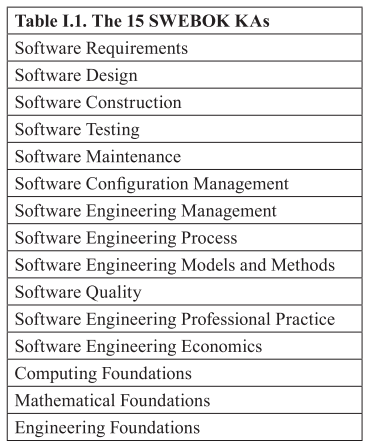
\includegraphics[width=\linewidth]{15KAs.png}
%   	\caption{The 15 Knowledge Areas (KAs) described in SWEBOK V3 [15]}
%   	\label{fig:KAs}
% \end{figure}


%We propose to categorize the StackOverflow data we obtain related to VA app development, into the 15 KAs. In this way we aim to categorize the challenges faced by VA app developers and may find certain KAs to contain more issues than others.

\subsection{Research Questions}
Our specific research questions are:
\begin{description}
\item [RQ1:]Under which SWEBOK KAs do Google Assistant and Alexa app developer StackOverflow posts, with at least 500 views, fall?
\item [RQ2:]Of these KAs, which ones contain posts with the most views?
\item [RQ3:]What are the demographics of posts within each identified SWEBOK KA?
\item [RQ4:]How do the number of posts, for \textit{all} of the identified SWEBOK KAs, change over time?
\item [RQ5:]How do the number of posts, in \textit{each} of the identified SWEBOK KAs, change over time?
\item [RQ6:]Are there any differences between StackOverflow questions on Amazon Alexa and Google Assistant, according to the SWEBOK taxonomy?
\end{description}

% \subsubsection{Hypotheses}
We hypothesize that some common challenges faced by VA developers will include:
\begin{enumerate}
\item Questions related to NLP and how to build good voice-based interfaces for these apps.
\item Bugs with software development kits.
\item Debugging issues.
\item Questions to better understand capabilities of software development kits. 
%(since most of these kits are still relatively new).
\end{enumerate}

% Additionally, we may see more people asking questions regarding VA apps from English speaking, developed countries, since most VAs primarily support English and are being sold in developed countries like the United States, Canada, and the United Kingdom.

\section{2. Methodology}
\subsection{Data Retrieval}
Software development data regarding VA app development can be obtained in many different ways. Interviews with open-ended questions are rich sources of qualitative and quantitative data because it is in natural language and can be used to compare development in different paradigms of software development \cite{1murphy2014cowboys}. The main caveat with conducting interviews is the limit on the number of interviewees, sampling bias in the selected sample of interviewees and cognitive biases in the researchers' interview questions. 

As of the time of writing, StackOverflow had more than 15 million questions and 8 million contributors. In comparison to similar Stack Exchange sites like Software Engineering Stack Exchange and Android Stack Exchange (which also contain valuable data on issues regarding software architecture, design and other knowledge areas), they contained a small portion of data with respect to StackOverflow (size of data was less than 300 times that of StackOverflow). Unlike popular generic discussion forums like Quora, StackOverflow downvotes posts, stimulating a matter of subjective opinion and encourages the sharing of factual matter. 
We initially restricted our scope to tags related to Alexa, Google Assistant, Siri, and Cortana based development issues because these 4 technologies are the most popular and prominent VAs as of the time of writing in March 2018. 

We used the Stack Exchange Data Explorer web tool for querying the data dump. We filtered the data using tags associated with the questions posted on StackOverflow. After an initial exploratory analysis, we found the most common tags associated with Google Assistant and Amazon Alexa to be those listed in Table \ref{table:tags}.

% \begin{table}[h!]
% \centering
%  \begin{tabular}{||m{11em} | m{11em}||} 
%  \hline
%  \textbf{Amazon Alexa} & \textbf{Google Assistant} \\ [0.5ex] 
%  \hline\hline
%  alexa-skills-kit & google-assistant-sdk  \\ 
%  \hline
%  alexa-voice-service & actions-on-google \\
%  \hline
%  alexa-slot & google-assist-api \\
%  \hline
%  alexa-skill & google-home \\
%  \hline
%  amazon-echo & google-smart-home \\  
%  \hline
% \end{tabular}
%  \caption{List of tags used to filter the StackOverflow data}
% \label{table:tags}
% \end{table}

\begin{table}[H] \tiny %place tables right after subheading and use H tag to force in under subheading%
\centering
%Resizebox encases the tabular tag to ensure we fit within a column%
\resizebox{\columnwidth}{!}{%
\renewcommand{\arraystretch}{0.9}% Tighter
\begin{tabular}{|l|l|}
\hline
\textbf{Amazon Alexa}          & \textbf{Google Assistant} \\ \hline
alexa-skills-kit & google-assistant-sdk            \\ \hline
alexa-voice-service & actions-on-google           \\ \hline
alexa-slot & google-assist-api           \\ \hline
alexa-skill & google-home           \\ \hline
amazon-echo & google-smart-home             \\ \hline
\end{tabular}
}
\caption{List of tags used to filter the StackOverflow data}
\label{table:tags}
\end{table}

We targeted the Posts table because we could then look into posts/questions which have high scores and are more frequently viewed, because that would reflect a prominent issue during VA app development. For each post we extracted the taglist, metrics related to activity such as score, comment count and number of views, and metrics related to the provenance of the issue like the last created and edited dates. 

\subsection{Data Processing}
Our empirical analysis is based on studying questions posted in StackOverflow pertaining to the ontology of principles that define the current state of VA app development. We study various attributes of the population of programming issues such as number of votes, number of views, and tags, to name a few. 
%Although this study is specific to VA technology, it spans a broad variety of terms ranging from prominent low-level difficulties in writing code and debugging API calls to the high-level organization of teams involved in building voice-assisted products. <- THIS IS ALREADY MENTIONED EARLIER IN THE PAPER

We separated the questions from the answers for each considered post for categorization and analysis. 
%We acknowledge this to be a threat to validity because although answers can possess important information, we thought that they could lead to misclassification of the content of the original post. 
After an initial exploratory analysis of our corpus, we found each question to possess multiple answers from multiple developers. Although the top rated answer was usually a direct solution to the problem, developers had provided alternative answers originating from different software design patterns or perspectives requiring different architectures. Hence, we formulated our categorization approach to depend on the question posted by the troubled developer him/herself. 
%This approach also benefited us with the increase in size and scope of the number of posts to be categorized. 
Attributes related to the creators and editors of posts were filtered out to eliminate the bias of prioritizing posts by user's profile level and contribution history. This bias refers to the study of those posts created and edited by high profile users since the underlying assumption is that these ``strongly contributing'' users tend to ask higher quality questions only after thorough research.

Based on the results from our exploratory study, we chose to look specifically at development regarding Google Assistant and Alexa primarily because of market maturity. HomePod, Apple's first independent VA, which used Siri, was released towards the end of 2017. This is relatively recent in comparison to its counterparts, Amazon Echo and Google Home. After examining our data, we concluded that the relatively short time period of developer activity regarding Siri may not offer valid insights on the progression and consistency of emergent trends over time. Microsoft's Cortana was not deployed on any stand-alone VA device at the time of writing. Therefore we restricted our data sample to posts related to existing VAs in stand-alone devices.  

\subsubsection{Hybrid Card Sort}
To categorize the retrieved StackOverflow posts into the 15 SWEBOK KAs, we started with a closed-card sort. We organized the rows of our data table according to the 'view count' metric, in descending order. We then proceeded to filter the data by view count--we set a cut off point of greater than or equal to 500 views; this left us with 303 posts, i.e. the top 303 most-viewed posts (of the data we retrieved). We decided to filter the data by view count because we wanted to start with the most 'popular' posts, and then see after categorizing the first 303, whether the posts were mainly being categorized into certain areas (i.e., we reached saturation) or whether the posts were being categorized in all different KAs. We found that after the first 303 posts, there were clear KAs into which most posts fell.

In terms of the post categorization process, we looked at the title and body of the post. If one of us found a post difficult to categorize, we would ask the other researchers to get their opinions. If a researcher felt a post did not fall into one of the 15 KAs, they classified the post as 'Other'. To maintain consistent categorization of posts amongst the 3 researchers, we started by categorizing the first 20 posts together. After this, each researcher categorized the next 10 posts individually, and then we compared our classifications. During the entire process, for any ambiguities, we discussed our view points and came to a conclusion on classification. Once we felt we were categorizing the posts in the same way, we partitioned the remaining posts and labelled the split data sets individually. 

Our method of categorization into SWEBOK KAs were based on our prior experience with software engineering. Programming errors and exceptions are an ubiquitous part of ''Software Construction'' and therefore were categorized as such. Posts related to design mechanisms of the application on various aspects of VA usage or development planning were categorized as ``Software Design'' issues. These not only included the design of response mechanisms with respect to user inputs, Intents, and Sample Utterances but also the methodology of integrating and deploying the VA app on different platforms such as web apps, or Google API integration. Although a Design issue could be related to other SWEBOK Areas such as Construction, a clear distinction between Design and Construction was made by the authors of the paper; posts were categorized as Design if the issue revolved around how to implement a certain aspect of the VA, and as Construction if the post had already found a way to implement but was struggling with successfully implementing that aspect. Posts labeled under the ``Software Testing'' SWEBOK KA fell into different forms of testing like local testing or simulator testing.  ''Software Configuration Management'' looked more towards the developer operations (DevOps) and preparation of an application for deployment, which may include the need for us to setup inclusions of any external APIs used before code can be compiled, and any issues in the deployment preparation process. This is the step when functional testing (which is covered in the Software Testing) is complete and for the most part, the application is ready to be released to end users.

After categorizing the top viewed 303 posts into the 15 KAs we split up the data further within each KA. Each researcher took a few of these KAs and for one KA at a time, read through each post again, assigning it to a subcategory which described its content representatively. The subcategories evolved as the researchers read through the posts. We decided to split the data according to KA to find the subcategories so that comparisons of posts could be made within one KA instead of across multiple KAs. 
We decided the themes of the subcategories based on emergent patterns in the issues because lower levels in the SWEBOK taxonomy do not accurately describe the collection of posts that we had, since VA app development is likely to have some unique activities that are typically not seen in traditional software development.

\section{3. Results}
Following the Hybrid Card Sorting process, we analyzed our data according to our Research Questions. This section will describe those analyses. Our aim is to highlight the most common issues experienced by VA app developers. By discovering these bottlenecks we may aid in the accelerated improvement, not only in VA technology and related API usage, but in application programming in general.

 \subsection{RQ1: Under which SWEBOK KAs do Google Assistant and Alexa app developer StackOverflow posts, with at least 500 views, fall?}

\begin{table}[H] %place tables right after subheading and use H tag to force in under subheading%
\centering
%Resizebox encases the tabular tag to ensure we fit within a column%
\resizebox{\columnwidth}{!}{%
\begin{tabular}{|l|c|}
\hline
\textbf{SWEBOK Knowledge Area}          & \textbf{Number of Posts} \\ \hline
Requirements                      & 0             \\ \hline
Design                            & 100           \\ \hline
Construction                      & 106           \\ \hline
Testing                           & 53            \\ \hline
Maintenance                       & 1             \\ \hline
Software Configuration Management (SCM)    & 21            \\ \hline
Engineering Management            & 0             \\ \hline
Engineering Process               & 0             \\ \hline
Engineering Models and Methods    & 0             \\ \hline
Quality                           & 0		      \\ \hline
Engineering Professional Practice & 0             \\ \hline
Engineering Economics             & 1             \\ \hline
Computing Foundations             & 0             \\ \hline
Mathematical Foundations          & 0             \\ \hline
Engineering Foundations           & 0             \\ \hline
Other                             & 21            \\ \hline
\rowcolor[HTML]{C0C0C0} 
\textbf{Total Number of Posts}                      & \textbf{303}  \\ \hline
\end{tabular}
}
\caption{Population Breakdown of Posts by SWEBOK KA}
\label{table:populationBreakdownSwebokKA}
\end{table}
 
The results in Table \ref{table:populationBreakdownSwebokKA} show the population breakdown into the SWEBOK KAs of the 303 categorized posts. A graphical representation of this result is also available in the appendix section in Figure \ref{fig:1PopulationBreakDownSwebok}.

As can be seen, the top 3 KAs found are Design, Construction and Testing. In the SWEBOK, \textit{Software Design} describes the movement from requirements to a description of implementation. It can include architecture design, interface design, and algorithm design, for example. \textit{Software Construction} defines the construction of the design components. \textit{Software Testing} includes unit testing, performance testing, system testing, etc. (For a comprehensive description of all SWEBOK KAs see \cite{hilburn1999software}).

The fact that we found the most common KAs in VA app development to be Design, Construction, and Testing is unsurprising as these are topics into which typical questions on a developer focused discussion forum like StackOverflow fall under. There were a number of posts that did not fit any of the SWEBOK KAs, and hence, were classified as `Other'. 
%We will be discussing the various subcategories that we identified under a particular SWEBOK KA in the subsequent sections of this paper. 

There was a noted absence of questions on StackOverflow regarding Engineering Practices (like Engineering Management, Engineering Process etc.) and the Software Engineering Foundations (i.e. Computing and Mathematical Foundations). This is interesting, as it likely indicates that there is less theoretical discussion going on in this sphere, compared to more practical and applied software engineering questions, that are directed towards how developers can build and test what they are working on for VAs. 

It is important to remember that this taxonomical breakdown into SWEBOK KAs was done on a pool of posts that each had at least 500 views. However, judging by the distribution and clear divide in the types of posts on StackOverflow on VA app development, we expect that these results would generalize if we were to repeat the same classification on all posts on StackOverflow that are related to VA app development.

\subsection{RQ2: Of these KAs, which ones contain posts with the most views?}
Based on the results of RQ1, we wanted to know which SWEBOK KA contained the posts with the most views. This was calculated by summing up the number of views for each post that was classified under a specific SWEBOK KA. The idea behind this is that in addition to understanding the population and landscape of posts, we would likely be able to see which SWEBOK KA was most popular, as it is possible that some KAs may have a small number of posts but a large view count, potentially suggesting many people had a similar question in that KA. 
%- and since the question had already been asked, these users did not have to re-ask the question on StackOverflow and would be an indication of a common problem being faced by many. Knowing this would allow providers of VA SDKs to be able to better understand common issues faced by developers using their SDKs.
\begin{table}[H] %DISABLED: place tables right after subheading and use H tag to force in under subheading%
\centering
%Resizebox encases the tabular tag to ensure we fit within a column%
%\resizebox{\columnwidth}{!}{%Disabled resize box here, re-enable if needed
\begin{tabular}{|l|c|}
\hline
\textbf{SWEBOK Knowledge Area}       & \multicolumn{1}{l|}{\textbf{Sum of Views}} \\ \hline
Design                & 189718                                     \\ \hline
Construction          & 166141                                     \\ \hline
Testing               & 88605                                      \\ \hline
SCM                   & 56254                                      \\ \hline
Engineering Economics & 1568                                       \\ \hline
Maintenance          & 8081                                       \\ \hline
Other                & 34171                                      \\ \hline
\end{tabular}
%}
\caption{Population Breakdown of Number of Views by SWEBOK KA}
\label{table:viewBreakdownAllSwebokKAs}
\end{table}
We present the results in Table \ref{table:viewBreakdownAllSwebokKAs} and a graphical representation of this data is provided in Figure \ref{fig:2ViewBreakDownSwebok} in the appendix of this paper. As expected, Design, Construction, and Testing, the 3 KAs with the largest number of posts (Table \ref{table:populationBreakdownSwebokKA}), also had the top 3 largest number of views. Interestingly, while the Construction KA has slightly more posts than the Design KA (Construction has 6 more posts than Design), it has a slightly smaller number of views. We note that while the SCM KA and the Other area both have the same number of posts, SCM has a significantly larger number of views than the Other area. This is likely because the questions in the Other area may not necessarily be questions that most people were looking for answers to, as opposed to the SCM area. This also happened in the case of Maintenance vs Engineering Economics, where both KAs have only one post respectively, but the Maintenance KA has over 5 times the number of views than the Engineering Economics KA. After further inspection we found that the question on Maintenance was mainly about deployment platforms while the question on Engineering Economics was about monetization opportunities in VA applications. We attribute this difference in view count to the nature of discussion on StackOverflow being a programming oriented site whereas alternative sites such as the Software Engineering Stack Exchange may contain more questions related to Engineering Economics.

\subsection{RQ3: What are the demographics of posts within each identified SWEBOK KA?}
%\textbf{ TODO DESIGN OF RQ3}
To better understand the situation in each specific SWEBOK KA identified, we calculated a summary of the subcategories. This allowed us to see if there were any noticeably pressing issues within a specific KA itself - an indication of an issue that seems to be experienced by many developers within a KA.

The results were summarized by SWEBOK KA, and then tabulated. We looked at a number of metrics, namely number of posts, number of views, number of comments, number of answers (answers are comments from the public that were found to be the answer to the post author's question, and are marked as such), and the number of favorites (the number of people who have favorited a particular post). For all tabulated data in this section, we have ordered them based on number of views.

\subsubsection{Software Design}
The most prominent difficulty found to be faced by Alexa and Google Assistant VA app developers in Software Design was due to the ``Controlling and Handling of Events'' followed by ``Error and Exception Handling and Fault Tolerance'' which had half the number of posts as the former design subcategory (Table \ref{table:DesignKASummary}). 

On further examination of the major design issues, we observe that developers face the highest difficulty in designing their VA app to handle boundary cases. This pertains to the programming of different algorithms by customizing Alexa slots to cover probable user responses and utterances during interactive dialogue  . Many developers also faced issues regarding account linkage and authentication APIs such as OAuth. Lack of support in terms of documentation and coding examples were also some of the reasons developers found difficulties with the Google Assist API.  

\begin{table}[H] %place tables right after subheading and use H tag to force in under subheading%
\centering
%Resizebox encases the tabular tag to ensure we fit within a column%
\resizebox{\columnwidth}{!}{%
\begin{tabular}{|l|c|c|c|c|c|}
\hline
\textbf{Subcategory} & \textbf{\begin{tabular}[c]{@{}c@{}}Number of\\ Posts\end{tabular}} & \textbf{\begin{tabular}[c]{@{}c@{}}Number of\\ Views\end{tabular}} & \textbf{\begin{tabular}[c]{@{}c@{}}Number of\\ Comments\end{tabular}} & \textbf{\begin{tabular}[c]{@{}c@{}}Number of\\ Favourites\end{tabular}} & \textbf{\begin{tabular}[c]{@{}c@{}}Number of\\ Answers\end{tabular}} \\ \hline
Control and Handling of Events & 38 & 72006 & 37 & 30 & 65 \\ \hline
\begin{tabular}[c]{@{}l@{}}Error and Exception Handling\\  and Fault Tolerance\end{tabular} & 11 & 30046 & 7 & 14 & 22 \\ \hline
\begin{tabular}[c]{@{}l@{}}How to build/implement \\ own skill\end{tabular} & 15 & 29476 & 12 & 16 & 26 \\ \hline
Security \& Authentication & 10 & 23474 & 4 & 31 & 23 \\ \hline
Distribution of Components & 15 & 17970 & 10 & 5 & 28 \\ \hline
\begin{tabular}[c]{@{}l@{}}Understanding voice\\  assistant SDK\end{tabular} & 3 & 6079 & 0 & 2 & 10 \\ \hline
API feature question & 5 & 5688 & 5 & 5 & 13 \\ \hline
3rd party SDK integration & 2 & 2940 & 2 & 1 & 4 \\ \hline
Disable/Block Google Services & 1 & 2039 & 2 & 6 & 3 \\ \hline
\end{tabular}
}
\caption{Summary of subcategories and their accompanying demographic information for the Design SWEBOK KA}
\label{table:DesignKASummary}
\end{table}

\subsubsection{Software Construction}
The subcategories found within the Construction KA are shown in Table \ref{table:ConstructionKASummary}. Interestingly, in comparison to the other KAs, the Construction KA contained posts across a wide range of topics. The top 6 most viewed subcategories will be discussed here. The top 3 most viewed subcategories are all based on Alexa Skill development. The top viewed posts are related to using AWS Lambda, a computing platform provided by Amazon Web Services, which aims to simplify building applications that respond to events and new information. 
%Users can upload their code to a Lambda function and Lambda will remove some of the complexity in setting up and managing an endpoint. AWS Lambda can accept code written in a number of different languages. 


\begin{table}[H] %place tables right after subheading and use H tag to force in under subheading%
\centering
%Resizebox encases the tabular tag to ensure we fit within a column%
\resizebox{\columnwidth}{!}{%
\begin{tabular}{|l|c|c|c|c|c|}
\hline
\textbf{Subcategory} & \textbf{\begin{tabular}[c]{@{}c@{}}Number of\\ Posts\end{tabular}} & \textbf{\begin{tabular}[c]{@{}c@{}}Number of\\ Views\end{tabular}} & \textbf{\begin{tabular}[c]{@{}c@{}}Number of\\ Comments\end{tabular}} & \textbf{\begin{tabular}[c]{@{}l@{}}Number of\\ Favourites\end{tabular}} & \textbf{\begin{tabular}[c]{@{}l@{}}Number of\\ Answers\end{tabular}} \\ \hline
AWS lambda function & 5 & 38474 & 9 & 7 & 12 \\ \hline
Alexa slots & 8 & 17609 & 9 & 3 & 15 \\ \hline
Amazon session attributes & 7 & 12890 & 7 & 6 & 12 \\ \hline
Audio issue & 6 & 11512 & 5 & 12 & 11 \\ \hline
http & 9 & 10929 & 12 & 2 & 9 \\ \hline
Alexa intent issue & 9 & 9173 & 6 & 5 & 15 \\ \hline
node.js & 3 & 7106 & 9 & 1 & 5 \\ \hline
Retrieving user information & 6 & 7075 & 2 & 4 & 10 \\ \hline
SSML & 6 & 6646 & 1 & 1 & 8 \\ \hline
\begin{tabular}[c]{@{}l@{}}Linking third party \\ info to Alexa skill\end{tabular} & 1 & 4088 & 3 & 3 & 1 \\ \hline
Using Alexa and cURL & 2 & 3380 & 2 & 1 & 6 \\ \hline
Responses & 4 & 3284 & 5 & 2 & 9 \\ \hline
Alexa skill state & 2 & 2749 & 1 & 1 & 3 \\ \hline
Preparing to test on Simulator & 3 & 2705 & 0 & 0 & 5 \\ \hline
Account linking & 3 & 2638 & 5 & 1 & 7 \\ \hline
api.ai & 3 & 2454 & 10 & 3 & 5 \\ \hline
\begin{tabular}[c]{@{}l@{}}How to implement\\ Google Assistant's\\ hotword.py\end{tabular} & 2 & 2356 & 1 & 0 & 4 \\ \hline
Device discovery alexa & 2 & 1938 & 3 & 2 & 6 \\ \hline
Raspberry pi & 3 & 1891 & 3 & 0 & 3 \\ \hline
gactions & 3 & 1884 & 0 & 1 & 6 \\ \hline
Google Assistant SDK and grpc & 1 & 1242 & 4 & 0 & 1 \\ \hline
Google Assistant installation & 1 & 1211 & 2 & 0 & 1 \\ \hline
Adding image to response card & 1 & 1192 & 0 & 0 & 2 \\ \hline
webhook & 2 & 1160 & 8 & 2 & 4 \\ \hline
\begin{tabular}[c]{@{}l@{}}ASK able to listen\\ on different ports\end{tabular} & 1 & 1147 & 0 & 0 & 1 \\ \hline
Custom actions & 1 & 1070 & 2 & 1 & 0 \\ \hline
\begin{tabular}[c]{@{}l@{}}Issue with Amazon Developer\\ Console -building interaction\\ model\end{tabular} & 1 & 1041 & 0 & 0 & 1 \\ \hline
Python & 1 & 941 & 0 & 0 & 1 \\ \hline
Dialog model & 1 & 849 & 1 & 0 & 1 \\ \hline
Changing Google Home voice & 1 & 706 & 0 & 0 & 1 \\ \hline
\begin{tabular}[c]{@{}l@{}}Communication with\\ own webservice\end{tabular} & 1 & 690 & 0 & 0 & 2 \\ \hline
Setting endpoint & 1 & 644 & 0 & 0 & 1 \\ \hline
Endpoint issue & 1 & 634 & 0 & 0 & 2 \\ \hline
Configuring ask-cli & 1 & 626 & 2 & 1 & 1 \\ \hline
State variables & 1 & 593 & 0 & 1 & 1 \\ \hline
Alexa utterances & 1 & 561 & 0 & 0 & 1 \\ \hline
Using OAuth2.0 server & 1 & 530 & 0 & 1 & 1 \\ \hline
\begin{tabular}[c]{@{}l@{}}Validation of \\ certificates chain\end{tabular} & 1 & 523 & 4 & 7 & 2 \\ \hline
\end{tabular}
}
\caption{Summary of subcategories and their accompanying demographic information for the Construction SWEBOK KA}
\label{table:ConstructionKASummary}
\end{table}

Posts about Alexa intents and slots were also highly viewed. When developing a Skill for Alexa, intents represent actions that fulfill a user's request. Intents include a name and a list of utterances that users are expected to say to invoke the intent. Slots are optional arguments that can be passed to intents. Slots are used as training data for Alexa's NLP, and therefore are important to building successful interaction models. 

Session attributes allow Alexa to store user-provided details during a session. The most viewed posts in this subcategory were about understanding how to use session attributes correctly. A number of posts were related to parsing and streaming audio files and converting mp3 files in both Alexa and Google Assistant contexts. Interestingly, all posts in the http subcategory were concerned with Alexa Skills development and most were on the topic of http request issues.

\subsubsection{Software Testing}
Based on the data presented in Table \ref{table:TestingKASummary}, it is clear that backend response issues were the main issue - this subcategory had the highest values across the board, indicating highest engagement and activity. The number of views on posts in this subcategory is not surprising, as by design, VAs depend a lot on backend communication which is often done on a remote server - the device merely acts as a light, frontend interface to the intelligence engine in the backend that makes sense of the request from a user and provides an appropriate response. 
\begin{table}[H] %place tables right after subheading and use H tag to force in under subheading%
\centering
%Resizebox encases the tabular tag to ensure we fit within a column%
\resizebox{\columnwidth}{!}{%
\begin{tabular}{|l|c|c|c|c|c|}
\hline
\textbf{Subcategory} & \textbf{\begin{tabular}[c]{@{}c@{}}Number of\\ Posts\end{tabular}} & \textbf{\begin{tabular}[c]{@{}c@{}}Number of\\ Views\end{tabular}} & \textbf{\begin{tabular}[c]{@{}c@{}}Number of\\ Comments\end{tabular}} & \textbf{\begin{tabular}[c]{@{}c@{}}Number of\\ Favourites\end{tabular}} & \textbf{\begin{tabular}[c]{@{}c@{}}Number of\\ Answers\end{tabular}} \\ \hline
\begin{tabular}[c]{@{}l@{}}Response issues\\ (Backend)\end{tabular} & 25 & 42868 & 32 & 16 & 47 \\ \hline
Local Testing & 8 & 12448 & 9 & 11 & 18 \\ \hline
Simulator Testing & 7 & 11342 & 14 & 4 & 17 \\ \hline
\begin{tabular}[c]{@{}l@{}}App compilation\\ issues\end{tabular} & 6 & 8943 & 5 & 1 & 7 \\ \hline
\begin{tabular}[c]{@{}l@{}}Response issues\\ (on device)\end{tabular} & 4 & 8348 & 7 & 6 & 7 \\ \hline
\begin{tabular}[c]{@{}l@{}}Response issues\\ (amazon slot)\end{tabular} & 1 & 2894 & 3 & 4 & 3 \\ \hline
Permission issues & 1 & 904 & 0 & 0 & 1 \\ \hline
\begin{tabular}[c]{@{}l@{}}Remote Data\\ publishing issues\end{tabular} & 1 & 858 & 4 & 0 & 2 \\ \hline
\end{tabular}
}
\caption{Summary of subcategories and their accompanying demographic information for the Testing SWEBOK KA}
\label{table:TestingKASummary}
\end{table}

Local and simulator testing issues were a close second, which is where developers try to push their code on to the local device or VA simulators online to test pseudo-real-world requests and responses. This too is particularly interesting and is quite unique to the development of intelligent agents like VAs, as they do not depend on visual interaction. It seems that the deployment for testing processes seems to be a bigger issue here than the response issues from the device, once the code is pushed - and is probably caused by uncertainty in the method and requirements to deploy to the simulator or to a local device. It may also be because of unreliability in the VA simulators.

\subsubsection{Software Configuration Management (SCM)}

\begin{table}[H] %place tables right after subheading and use H tag to force in under subheading%
\centering
%Resizebox encases the tabular tag to ensure we fit within a column%
\resizebox{\columnwidth}{!}{%
\begin{tabular}{|l|c|c|c|c|c|}
\hline
\textbf{Subcategory} & \textbf{\begin{tabular}[c]{@{}c@{}}Number of\\ Posts\end{tabular}} & \textbf{\begin{tabular}[c]{@{}c@{}}Number of\\ Views\end{tabular}} & \textbf{\begin{tabular}[c]{@{}c@{}}Number of\\ Comments\end{tabular}} & \textbf{\begin{tabular}[c]{@{}c@{}}Number of\\ Favourites\end{tabular}} & \textbf{\begin{tabular}[c]{@{}c@{}}Number of\\ Answers\end{tabular}} \\ \hline
Software questions & 13 & 43952 & 17 & 17 & 26 \\ \hline
Documentation concern & 1 & 4761 & 0 & 1 & 4 \\ \hline
API questions & 4 & 2915 & 0 & 0 & 6 \\ \hline
Hardware setup issue & 2 & 2796 & 0 & 0 & 2 \\ \hline
Environment issues & 1 & 1830 & 2 & 1 & 4 \\ \hline
\end{tabular}
}
\caption{Summary of subcategories and their accompanying demographic information for the Software Configuration Management (SCM) SWEBOK KA}
\label{table:SCMKASummary}
\end{table}
Software Configuration Management (SCM), whose definition is more towards the final deployment and preparation for release to market of an application, was a relatively small pool in our sample. However, within this small pool, we noticed that most of the issues were typically (unsurprisingly) related to software questions, specifically towards the preparation of the software being developed for final deployment, or issues in the deployment process. Interestingly, there were a lot of views for the single post on documentation concerns, where there were concerns raised due to unclear documentation in the SDK. SDK providers should therefore make sure issues in the documentation of their SDKs are solved and are as clear as possible as it seems to be an issue many are experiencing.

\subsubsection{Engineering Economics}

\begin{table}[H] %place tables right after subheading and use H tag to force in under subheading%
\centering
%Resizebox encases the tabular tag to ensure we fit within a column%
\resizebox{\columnwidth}{!}{%
\begin{tabular}{|l|c|c|c|c|c|}
\hline
\textbf{Subcategory} & \textbf{\begin{tabular}[c]{@{}c@{}}Number of\\ Posts\end{tabular}} & \textbf{\begin{tabular}[c]{@{}c@{}}Number of\\ Views\end{tabular}} & \textbf{\begin{tabular}[c]{@{}c@{}}Number of\\ Comments\end{tabular}} & \textbf{\begin{tabular}[c]{@{}c@{}}Number of\\ Favourites\end{tabular}} & \textbf{\begin{tabular}[c]{@{}c@{}}Number of\\ Answers\end{tabular}} \\ \hline
\begin{tabular}[c]{@{}l@{}}Monetization \\ opportunities\end{tabular} & 1 & 1568 & 0 & 0 & 2 \\ \hline
\end{tabular}
}
\caption{Summary of subcategories and their accompanying demographic information for the Engineering Economics SWEBOK KA}
\label{table:EEKASummary}
\end{table}
As seen in Table \ref{table:EEKASummary}, there was only one post categorized as Engineering Economics (EE) and it was related to monetization opportunities in VAs. This is not very surprising as StackOverflow by nature is a technical site and is often a place where developers go when they have a technical question about something they are working on. Nevertheless, there was still a large number of views on this single post, indicating there is some interest in this area as well.
\subsubsection{Software Maintenance}
\begin{table}[H] %place tables right after subheading and use H tag to force in under subheading%
\centering
%Resizebox encases the tabular tag to ensure we fit within a column%
\resizebox{\columnwidth}{!}{%
\begin{tabular}{|l|c|c|c|c|c|}
\hline
\textbf{Subcategory} & \textbf{\begin{tabular}[c]{@{}c@{}}Number of\\ Posts\end{tabular}} & \textbf{\begin{tabular}[c]{@{}c@{}}Number of\\ Views\end{tabular}} & \textbf{\begin{tabular}[c]{@{}c@{}}Number of\\ Comments\end{tabular}} & \textbf{\begin{tabular}[c]{@{}c@{}}Number of\\ Favourites\end{tabular}} & \textbf{\begin{tabular}[c]{@{}c@{}}Number of\\ Answers\end{tabular}} \\ \hline
Platform to deploy & 1 & 8081 & 0 & 3 & 2 \\ \hline
\end{tabular}
}
\caption{Summary of subcategories and their accompanying demographic information for the Maintenance SWEBOK KA}
\label{table:MaintenanceKASummary}
\end{table}
This KA attempts to primarily address post release development work. That is, once an app is out for public use, how a developer can extend the features of the application, deploy the same application on a different platform, and support the application. As this area of development is still very new, we did not expect to see many questions in this category. In fact, based on Table \ref{table:MaintenanceKASummary}, we only have a single post in this category, related to deployment platforms. This post was mainly looking at ways to port one implementation over from one platform to another, which is something some developers who have been successful in deploying for one VA platform would be considering to do. In fact, for just a single post, there is a relatively high view count, at just over 8000 views. We expect more questions in this area to appear over time as VA development becomes more mature.

\subsubsection{Other}
\begin{table}[H] %place tables right after subheading and use H tag to force in under subheading%
\centering
%Resizebox encases the tabular tag to ensure we fit within a column%
\resizebox{\columnwidth}{!}{%
\begin{tabular}{|l|c|c|c|c|c|}
\hline
\textbf{Subcategory} & \textbf{\begin{tabular}[c]{@{}c@{}}Number of\\ Posts\end{tabular}} & \textbf{\begin{tabular}[c]{@{}c@{}}Number of\\ Views\end{tabular}} & \textbf{\begin{tabular}[c]{@{}c@{}}Number of\\ Comments\end{tabular}} & \textbf{\begin{tabular}[c]{@{}c@{}}Number of\\ Favourites\end{tabular}} & \textbf{\begin{tabular}[c]{@{}c@{}}Number of\\ Answers\end{tabular}} \\ \hline
Account Setup & 7 & 13424 & 2 & 10 & 11 \\ \hline
Non Developmental & 4 & 11751 & 0 & 22 & 8 \\ \hline
\begin{tabular}[c]{@{}l@{}}Skill Management \\ (Add/Remove from\\ device)\end{tabular} & 2 & 1997 & 2 & 0 & 1 \\ \hline
\begin{tabular}[c]{@{}l@{}}Invoke Assistant \\ question\end{tabular} & 1 & 1680 & 0 & 0 & 2 \\ \hline
Hardware Options & 1 & 1638 & 4 & 1 & 2 \\ \hline
\begin{tabular}[c]{@{}l@{}}Speech language \\ question\end{tabular} & 2 & 1353 & 2 & 2 & 3 \\ \hline
\begin{tabular}[c]{@{}l@{}}Developer Console \\ user instructions\end{tabular} & 2 & 1266 & 3 & 0 & 2 \\ \hline
\begin{tabular}[c]{@{}l@{}}Deployment - \\ non conventional\end{tabular} & 1 & 561 & 0 & 0 & 1 \\ \hline
Build Ideas & 1 & 501 & 0 & 0 & 1 \\ \hline
\end{tabular}
}
\caption{Summary of subcategories and their accompanying demographic information for the Other SWEBOK KA}
\label{table:OtherKASummary}
\end{table}
The most viewed and highest number of posts in the Other category were on the topic of ''Account Setup''; more specifically the majority were on linking an account with the Google Assistant Action. The most viewed post in that subcategory was on retrieving a unique device id to be linked with the Action. The posts categorized as Non-Developmental were varied: running Amazon Echo within a private network, making the Google Actions development project preview persist longer, and a question about being able to launch an Alexa skill with just the name of the skill. The rest of the posts covered starting-up Google Assistant programatically, questioning where the console is when using AWS Lambda, and deploying a Google Action without it being publicly available. 

\subsection{RQ4: How do the number of posts, for \textit{all} of the identified SWEBOK KAs, change over time?}
\subsubsection{Growth in the number of posts, for posts with at least 500 views}
In addition to looking into the demographic data, we were also interested in how the number of posts increased over time. Unfortunately, we were not able to obtain historical data of the number of views on a particular post. Instead, we were only able to get the latest view count of a particular post. As a result, we decided to use the increase in the number of posts related to VA app development to see how this area has grown over time on StackOverflow, and is an indication of developer activity.

We first looked at this from the perspective of posts with at least 500 views, just as in the prior sections of this paper. The results we obtained can be seen in the graphs in the appendix section - \ref{fig:3GrowthInNumPosts500Views} and \ref{fig:3.1RateGrowthInNumPosts500Views}, which both show the growth in the number of posts, as well as the monthly rate of growth in the number of posts over time, for posts with at least 500 views. For better detail, a tabulated version of the same data is available in Table \ref{table:GrowthRateAndGrowth500Views}, also in the appendix of this paper.

There is no activity until June 2015, when we see the first two posts coming in. The rate of growth is seen to be relatively low, between June 2015 - November 2015. However, we do see a spike in the rate of growth in December 2015, and this rate of growth almost steadily increases until June 2016, when a large spike in the rate of growth occurs. This seems pretty consistent with the fact that Amazon Alexa was launched initially in November of 2014, but only hit the mass market in June of 2015, and the holiday season of 2015 would have likely caused the spike at the end of 2015, as people started to get their hands on Alexa powered devices like Amazon Echo.

Google's Assistant platform was introduced in mid-May 2016, and the first Assistant powered devices like Google Home only entered the market in early November 2016. There seems to be an initial spike in the number of new posts in June 2016, coinciding very closely to Google Assistant's launch and while the spike drops off in July 2016, the rate of growth (denoted by the number of new posts per month) steadily increased before an exponential increase between October - December 2016 as both Google Home and Amazon Echo were available on the market. Once again, we see a post December drop (after the holiday season), before it starts to pick up again between March - May 2017. 

Interestingly, we noticed a drastic drop in the rate of growth, where the number of new posts per month dropped significantly after May 2017. This wasn't expected initially, since there seemed to be a general view based on the data that the number of posts over time were steadily increasing (noted by the smooth curve of increase in Figure \ref{fig:3GrowthInNumPosts500Views}, before it tapers off). As a result, we decided to investigate the drop in the rate of growth of the number of posts by looking into the entire population, and not only posts which had at least 500 views. We suspected that part of the reason for why posts that were created after May 2017 did not appear in our observation here was because many of them may not have reached the required 500 view mark, and as a result, were not included in these graphs.

\subsubsection{Growth in the number of posts, regardless of view count}
We studied the rate of growth in the number of posts per month, as well as the growth curve of posts related to VA app development. 
Table \ref{table:GrowthRateAndGrowthAllViews}, in the appendix of this paper shows us the monthly growth rate (denoted by the number of new posts per month), as well as the sum of the number of posts at the end of every month. As seen in the graphical representation of the increase in number of posts and growth rate in  Figures \ref{fig:4GrowthInNumPostsAllViews} and \ref{fig:4.1RateGrowthInNumPostsAllViews}, 
we observe a rapid increase in the number of posts over time. This is further supported by the exponential increase in the rate of growth over time, for the most part. Oddly there is an unexplained sharp drop in the rate of growth for the month of September 2017, compared to August and October 2017, but in general, the momentum carried up to August 2017 carries on after October 2017.

We note there is a sharp drop in the number of new posts in the month of March 2018, leading to tapering off in the number of posts over time at the end of Figure \ref{fig:4GrowthInNumPostsAllViews}. We attribute this to the fact we extracted our corpus in March 2018, which does not spare enough time for the discovery of new bugs and issues.
Nevertheless, it does prove that there is a significant growth in the number of posts over time, indicating strong developer activity in this field, since the number of new questions developers are posting are increasing sharply over time. It also proves the reason we noticed a tapering off in the growth in Figure \ref{fig:3GrowthInNumPosts500Views}, which was mainly because posts after May 2017 were still relatively new and did not reach the 500 views cutoff we had when we sampled. This exponential growth provides us motivation to continue further research into the problems that developers face in the development of VA apps.

\subsection{RQ5: How do the number of posts, in \textit{each} of the identified SWEBOK KAs, change over time?}
In addition to looking at activity in general, we looked at activity by SWEBOK KA, as we wanted to see when a particular SWEBOK KA became active with regards to VA app development, and understand how active that particular KA was over time. 
%Additionally, we could find whether any particular SWEBOK KA experienced exponential growth, indicating that numerous problems related to that particular SWEBOK KA were faced by many developers at the same time. 
We would also be able to see if there were any patterns in when a specific SWEBOK KA became active (i.e. Design KA becoming active before the Construction KA - which is consistent with a typical software engineering life cycle).

We initially decided to look into the activity for each of the SWEBOK KAs, however once we obtained data, we realized that with the rule we set where a post had to have at least 500 views before it was included in our sample, the Engineering Economics, Software Configuration Management (SCM), Maintenance, and Other KAs did not have a sample large enough to draw any convincing conclusions %(these KAs had at most 21 posts that could be studied, in the case of the SCM KA and Other KA, while Engineering Economics and Maintenance only had 1 post each). 
As a result, we decided to focus on the 3 KAs with a large enough sample, namely Design (100 posts), Construction (106 posts), and Testing (53 posts).

\subsubsection{Design (100 posts)}
We refer to the Figures \ref{fig:5DesignGrowthInNumPosts500Views} and \ref{fig:5.1DesignRateGrowthInNumPosts500Views} in the appendix of this paper, which shows us the monthly growth rate (represented by the number of new posts per month) and the cumulative number of posts over time. We note that for the most part, the growth curve for the Design KA seems to be very similar to the growth curve of the entire sample of posts with at least 500 views. In fact, the growth rate pattern for Design KA (shown in Figure \ref{fig:5.1DesignRateGrowthInNumPosts500Views}) looks relatively similar to the growth rate pattern for the entire sample of posts with at least 500 views (as per Figure \ref{fig:4.1RateGrowthInNumPostsAllViews}). We start seeing posts come in as early as July 2015, making the Design KA posts to be one of the earlier posts that come up on StackOverflow for VA app development. This would be expected and is consistent with the idea that people would be running into design issues much earlier than other KAs, as the Software Design process is one of the earlier steps in a typical software development process. We do see the tapering off in the growth curve towards the end of 2017, which again is likely attributed to the fact that newer Design KA posts had not reached the 500 view count requirement to be included in our sample. This similar observation was made when looking at the growth curve of posts when the entire sample of posts with at least 500 views was considered.

\subsubsection{Construction (106 posts)}
We refer to the Figures \ref{fig:6ConstructionGrowthInNumPosts500Views} (growth curve) and \ref{fig:6.1ConstructionRateGrowthInNumPosts500Views} (rate of growth) in the appendix of this paper. We found that the general pattern of growth seems quite similar to the general pattern of growth of the sample of posts with at least 500 views, however when the pattern of growth of the Construction KA is compared to the Design KA, it is not as steep, as the growth for Construction KA is a bit more spread out. This is likely due to the fact that the software construction process is more prolonged and spread out over time, compared to the design process. Tapering off at the end of 2017 is again attributed to the fact that newer posts may not have reached the 500 view count level and hence were not included in our sample. 

\subsubsection{Testing (53 posts)}
Referring to the graphical representation of the data in Figures \ref{fig:7TestingGrowthInNumPosts500Views} and \ref{fig:7.1TestingRateGrowthInNumPosts500Views} in the appendix of the paper, it is interesting to see that the growth curve here is not as smooth as the base sample of posts with at least 500 views, or the growth curve of the Design or Construction KAs. There are a number of flat spots in the curve in the early stages up to March 2016, before it starts to increase somewhat uniformly. The reason for flat spots is most likely due to the testing problems and questions not being usually asked in the early stages of software development and is likely to be a topic of concern later on in a development cycle. Early questions are few and sporadic and most likely question on how people can test their code and implementations, as people start to prepare for testing and experience testing issues.
\subsubsection{Summary}
For the most part, the SWEBOK KAs investigated here seem to exhibit a similar growth curve as the general growth curve of all posts with at least 500 views. It is interesting to note that testing questions only became prevalent later than the design and software construction, which is similar to the order of activities in the typical development process. Naturally not all questions will be asked or answered, but it is good to know there is still an exponential growth of questions (based on the growth curves) in specific KAs as well, meaning there are more questions and pretty high levels of activity in this area as time goes on.

\subsection{RQ6: Are there any differences between StackOverflow questions on Amazon Alexa and Google Assistant, according to the SWEBOK taxonomy?}
Thus far, we have only looked at posts regarding Google Assistant and Alexa as one, and not differentiating them. However, we also wanted to see whether a particular platform had any difference in terms of number of posts per SWEBOK KA or in growth of the number of posts over time. We begin by looking at a breakdown of posts related to a particular platform, and grouping them based on the assigned SWEBOK KA to the post. A graphical representation of our findings is in the appendix, Figures \ref{fig:AlexaPostsSWEBOK} and \ref{fig:GAPostsSwebok}. In both cases, the Design, Construction and Testing KAs were the top 3 KAs for posts, with Google Assistant having a few more Design KA posts compared to Construction KA posts, while Alexa had a few more Construction KA posts than Design KA posts - however the differences were not major. 11.71\% of posts on Google Assistant were related to SCM, while only 4.17\% for Alexa, which was rather surprising. There were also a significantly larger proportion (11.71\% vs 4.17\%) of posts in Google Assistant that fell in the Other KA, indicating there were more questions that were not directly related to any existing defined SWEBOK KA for this platform, compared to Alexa. There was a slightly larger proportion of posts related to Testing for Alexa compared to Google Assistant, but this size difference isn't particularly large. On the whole, out of the 303 posts with at least 500 views, 192 posts (63.36\%) were related to Alexa, while 111 (36.63\%) were related to Google Assistant. This may not be wholly representative of the entire population, as we only looked at posts with at least 500 views. 

We decided to also look at how the posts for both platforms grow over time. The Alexa growth curves are available in Figures \ref{fig:8AmazonGrowthInNumPosts500Views} and \ref{fig:8.1AmazonRateGrowthInNumPosts500Views}, while the Google Assistant growth curves are available as Figures \ref{fig:9GAGrowthInNumPosts500Views} and \ref{fig:9.1GARateGrowthInNumPosts500Views} in the appendix of this paper. The biggest difference between the two platforms in terms of growth curves is the fact that while the Alexa growth curve was smoother and resembled the general growth curve of the sample of posts with at least 500 views (refer to Figure \ref{fig:3GrowthInNumPosts500Views}), the Google Assistant curve in Figure \ref{fig:9GAGrowthInNumPosts500Views} is relatively flat until November 2016 when it begins a sharp rise. This is consistent with the fact that it was around this time that Google Assistant and the first devices that ran Google Assistant independently, like Google Home, entered the mass market. We note that towards the end of the curves for both platforms, there is a pattern that indicates tapering off (a reduction in the rate of growth), but this is likely attributed to the fact that newer/younger posts may not have reached the 500 view count level to be included in our sample. Both platforms have pretty high levels of activity, indicating that both platforms contributed to our sample.
%and if at all, Google Assistant has a much spikier rate of growth compared to Amazon Alexa.

\section{4. Discussion}
Although VA app development varies from different platforms to programming languages, devices and companies, the cognitive aspect of a VA must remain constant. Ideally, VAs must be able to process natural language and execute actions reliably without negative consequences. In our study, we highlight the most common issues of VA app development with respect to each SWEBOK KA and suggest alternative methodologies so that product architects, development managers and developers themselves orient towards a common mindset. This not only triages issues for future work but also promotes the integration of different VAs and platforms seamlessly.

Our analyses indicated the following main issues in designing VA apps from a developer's perspective:
\begin{itemize}
\item Handling user input/output
\item Integrating Alexa with mobile-web-apps using third-party APIs
\item Working around Privacy or Account issues
\item Running on a particular platform ( Raspberry pi or Android for example)
\item Customizing Alexa slots
\end{itemize}
%We also found developers faced difficulties in dealing with audio and converting MP3 files. Although this could hint that VA users are interested in apps producing music, our findings from observing the most relevant issues in Software Construction showed only a few posts (2 out of 303) on MP3 files and audio clips. 

The most viewed posts classified as Other were regarding account linking with Google Assistant Actions. This is probably something Google could improve on, in the way they have their user guides with regards to account setup procedures. The most common issues categorized under Software Testing were related to backend response issues, as well as local and simulator testing. This is similar to the findings of \cite{4joorabchi2013real} who found that developers for mobile apps lacked robust monitoring, analysis, and testing tools. From the perspective of SCM, the main questions were on the preparation of the software developed for deployment purposes. The documentation concerns also highlighted is something that SDK platform providers like Amazon and Google could solve by making parts of their documentation clearer to developers. 
There is scope for  improvement with feedback based approaches, such as the ``Alexa Dev Tips'' skill \cite{AlexaDevTips}, which is designed to connect Alexa developers with news, tips, and resources for building skills. Dev Tips uses Skill Builder Entity Resolution for determining whether Alexa has an answer to a question or a ``miss''. By logging the slot values in the database, the skill prioritizes users' requirements and continuously improves the VA's response mechanism
\subsection{Future Work}
The biggest takeaway from this study is how similar the top SWEBOK KAs identified in this study, regardless of platform, are to the general software development process - that is, just like in traditional development, design, construction and testing are the typically most important steps and have the most number of pain points. It is also interesting to see that within a particular SWEBOK KA, especially Design, Construction, and Testing, we notice the subcategories within them are relatively unique to VA app development. This indicates that while on the surface the general problem areas may be similar, when examined more closely, VA app development has it's own unique set of problems, and many of these are problem are not seen in other types of software development.

One of the most highly viewed posts in our data set was due to \textbf{``lack of documentation''} when using Google Assist API. The developer intended to create his/her own assistant app by integrating other APIs with Google Now and Android but complained of a lack of documentation. The general intuition is for programmers to explore documentation online and then query StackOverflow if they do not find answers to their questions. Release of fully updated documentation, synchronized with correct release snapshots will accelerate the resolution of issues and contribute to a seamless integration of various APIs, thereby making VA app development more attractive and painless.

There is undoubtedly exponential growth in the number of questions being posted on forums like StackOverflow with regards to VA app development. The sheer activity of users posting questions about VA app development is an indication of activity in the VA app development sphere, and also an indication that there is an ever increasing number of issues and concerns being experienced by VA app developers. As the number of VA platforms increase over time, such as SiriKit for Apple's HomePod and Microsoft Cortana on stand-alone devices, we would expect the rate of issues and concerns being experienced by developers to increase. It would be interesting to see how the types of issues may develop over time as additional platforms are introduced.

How quickly and effectively platform providers like Amazon and Google solve the common issues highlighted in this study will be one of the contributors to the success and/or failure of a platform. If a platform provider like Amazon or Google ignores the problems and issues developers face when building for the particular VA platform, and if these problems are severe enough, 
%and require developers to come up with various hacks and workarounds, 
new developers will likely shy away from starting to develop on that particular platform, and existing developers may phase out their existing efforts if it becomes too costly and time-consuming to deal with the problems they face. The converse of this is true as well; if a platform provider actively improves their resources and SDKs and understand and alleviate developer issues, they are more likely to gain a strong following from independent 3rd party developers to build apps for their platforms. This is likely to make a platform more diverse in terms of available 3rd party services that work with that particular platform, making that platform more attractive to end users - especially those who may be interested in choosing between two devices on different platforms.

\section{5. Threats to Validity}
We acknowledge a number of threats to the construct validity of our study. First, we did not include the answers contributed by the public to the posts considered. Although answers carry vital information pertaining to different SWEBOK KAs, our intuition was that the content of answers may lead us to mis-classify the posts. 

Second, our analyses are based only on posts pertaining to Google Assistant and Alexa app development. We acknowledge that we therefore did not look at all VA app development currently taking place, however since Microsoft's Cortana does not currently exist within a stand-alone VA device, and Apple's Homepod was released at the end of last year, the most mature VA app development communities from which we could access sufficient data were Google Assistant and Amazon Alexa. We plotted and compared the number of issues faced by developers over time with Google Home, Alexa, Siri, and Cortana and observed a rising trend in the number of posts created per month in Google Home and Alexa. This was done for all related StackOverflow ``tags'' for the VA app development although figure \ref{fig:11MonthlyPostsforAGSC} shows the 3 most relevant tags. Siri and Cortana did not show an increase since the inception of their VA app development platforms. Therefore we chose to focus only on Alexa and Google Home due to the abundance of quantitative and qualitative data on improving VA app engineering. As we found clear similarities between the sizes of the posts and content of the two platforms and defined SWEBOK KAs for both, we believe the results are generalizable beyond the VA platforms studied here.  

Third, although our sub-sampling of posts with at least 500 views could threaten the validity of our study, the motivation for this paper lies in finding the most common issues faced by VA app developers. Looking at posts with fewer than 500 views would not have provided us with any significant information. 

Fourth, by using a hybrid card sorting process, we introduced the possibility of cognitive bias and human error. We attempted to mitigate this by making sure all researchers were categorizing posts in a similar way and all were familiar with and understood the definitions of the KAs. Additionally, all posts were categorized twice, once for the KA and once for the subcategories. 
% We hypothesized that we would see more people asking questions regarding VA app development from English speaking, developed countries. Unfortunately we were unable to access and analyze this data, however we believe that it is possible that posts on StackOverflow are biased to these regions of the world considering that these platforms have been mainly available in English speaking markets the longest, and only recently have been introduced in countries with English not being the primary language. 

Lastly, our data was retrieved from only one site, StackOverflow. We did not use Google and Amazon developer sites or other Stack Exchange Sites. This could introduce a bias as there may be only certain people who use StackOverflow, or ask certain types of questions on StackOverflow, which may be different on the other sites.
\section{6. Conclusion}
In this study we found the most common challenges faced by Google Assistant and Alexa app developers according to the SWEBOK KAs. Further research is needed to see how these problem areas evolve over time, and ideally this will help platform providers, like Amazon and Google, better tailor their SDKs and accompanying documentation and support services to help improve the developer experience.
\section{7. Dataset Availability}
We are making this dataset available on GitHub for readers of this paper at \url{https://github.com/kapilharesh/W18_CS846-Empirical_SE_VoiceAssistants}.
{\footnotesize \bibliographystyle{IEEEtranS}
\bibliography{reference}}
\pagebreak
\onecolumn %we use this tag to allow us to have one column formatting here%
\section {8. Appendix}
\begin{figure}[ht] %use the h (here) and t (top) tag%
	\centering %Ensure an image is centered%
	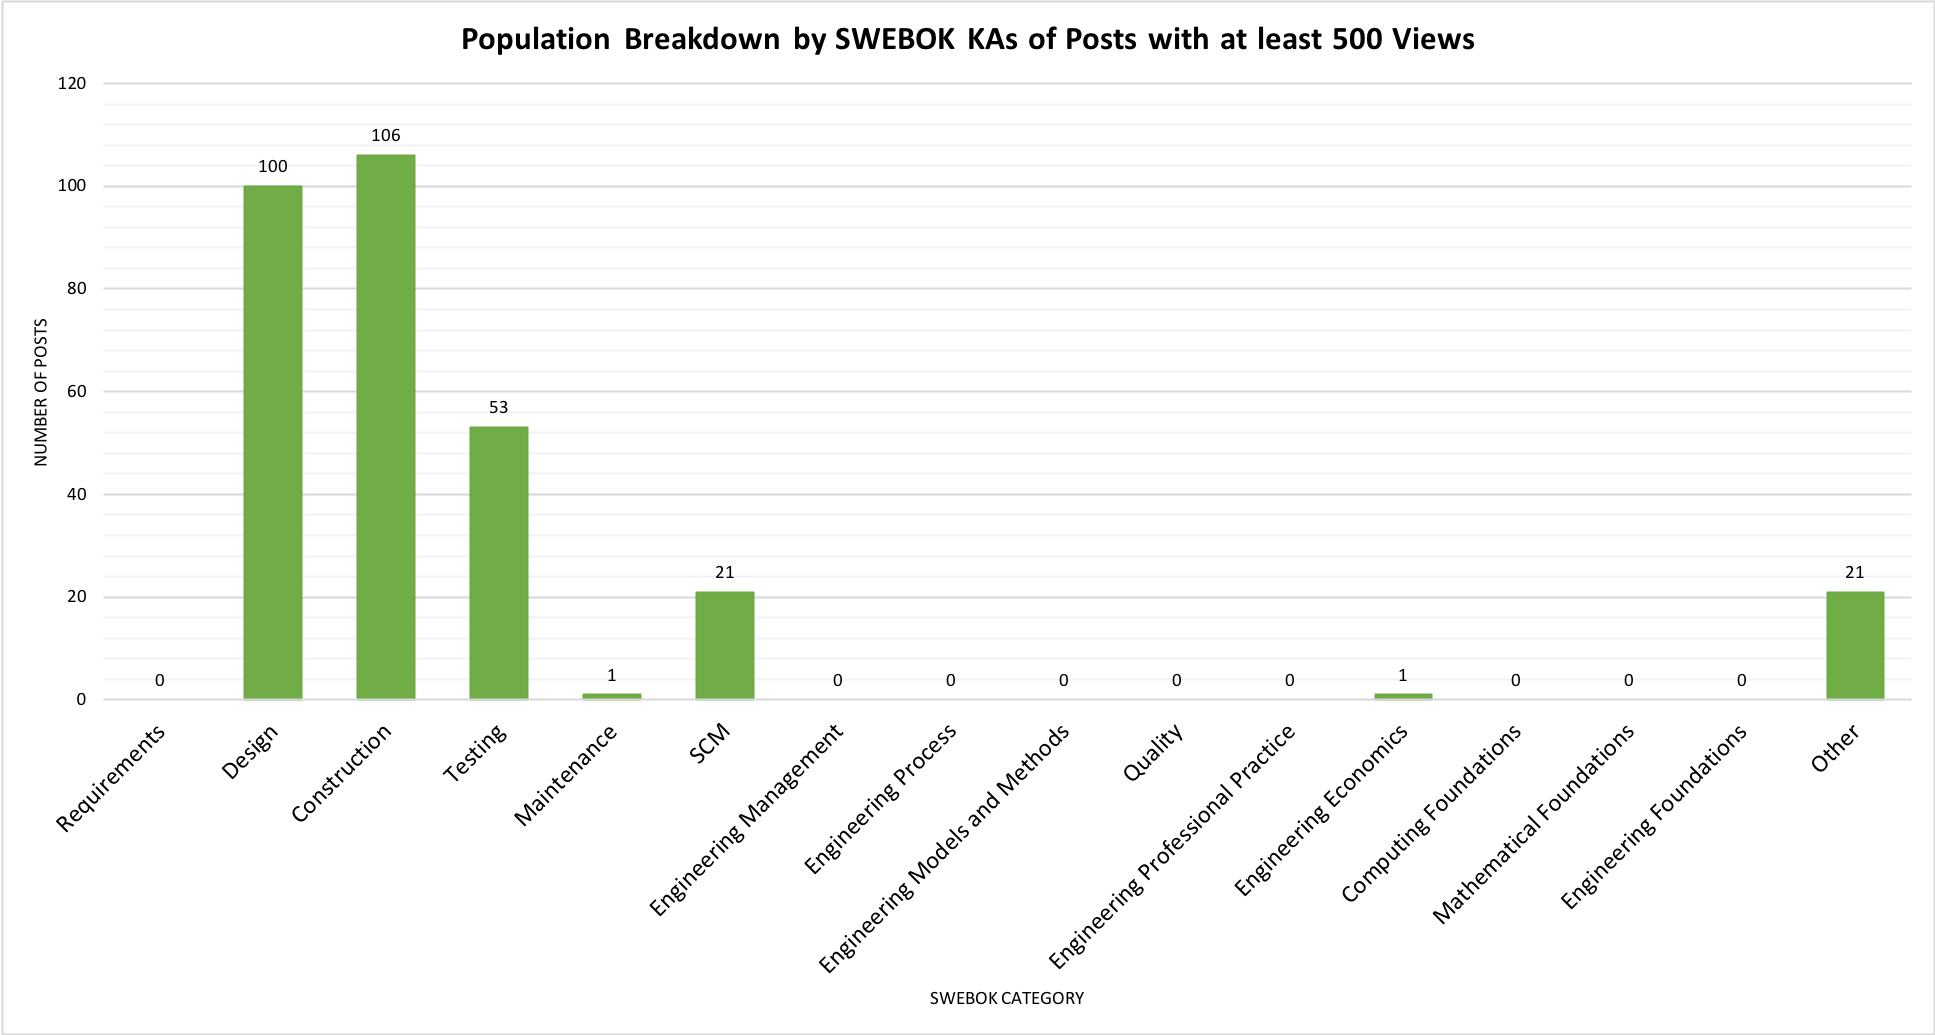
\includegraphics[width=0.8\textwidth,height=0.7\textheight,keepaspectratio]{RQ1_Size_of_Each_SWEBOK_Cat.png}%adjust the ratios to ensure images fit%
    \caption{Population breakdown by SWEBOK KAs for posts with at least 500 views}
    \label{fig:1PopulationBreakDownSwebok}
\end{figure}
\begin{figure}[ht]
	\centering
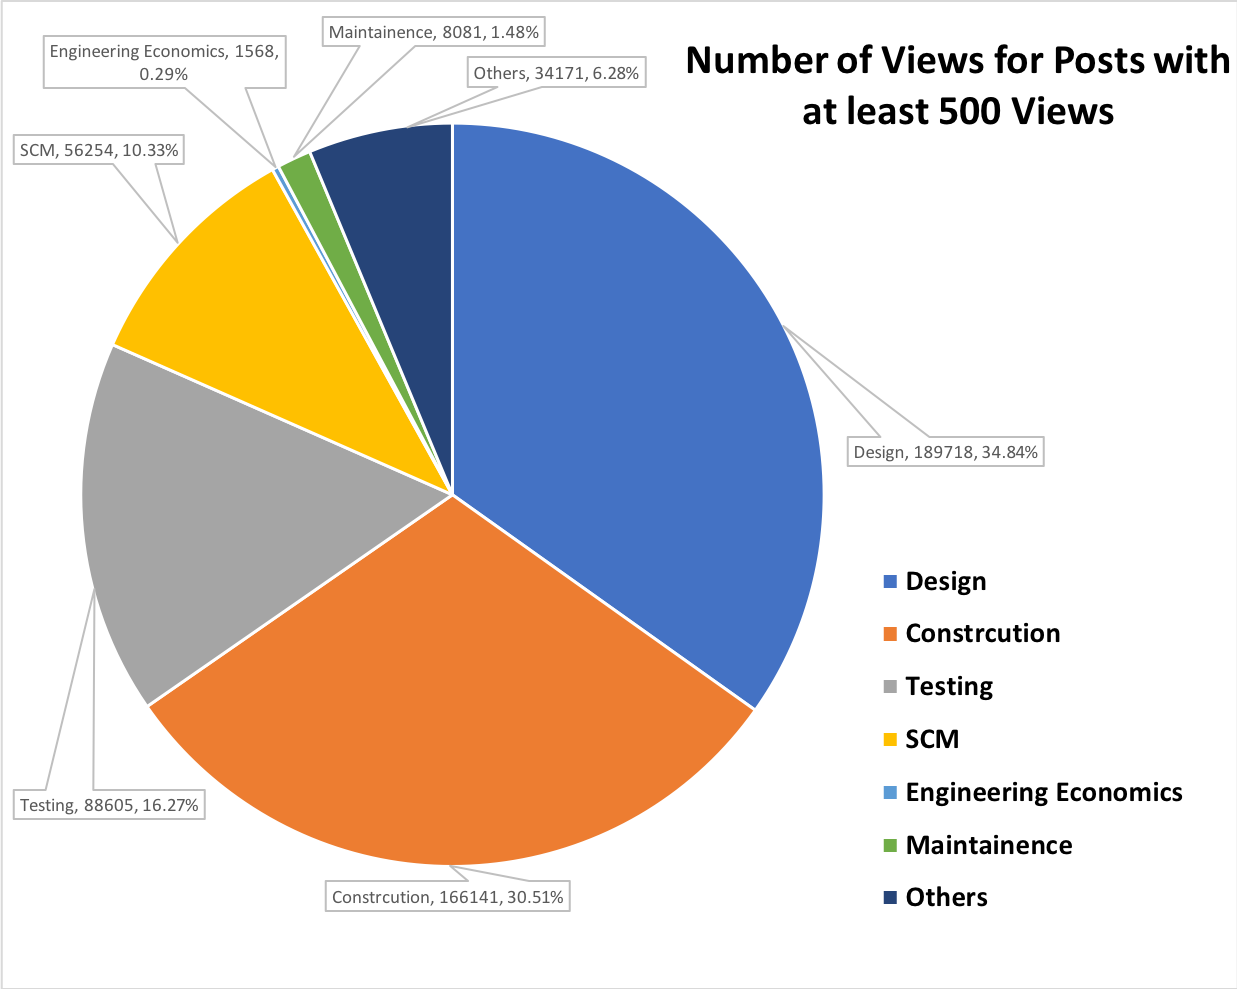
\includegraphics[width=0.55\textwidth,height=0.55\textheight,keepaspectratio]{RQ2_NumViewsPostsAll.png}
    \caption{Breakdown of number of views, by SWEBOK KA, for posts with at least 500 views}
    \label{fig:2ViewBreakDownSwebok}
\end{figure}
\pagebreak
\begin{table}[H] %place tables right after subheading and use H tag to force in under subheading%
\centering
%Resizebox encases the tabular tag to ensure we fit within a column%
\resizebox{\columnwidth}{!}{%
\begin{tabular}{|c|l|c|c|}
\hline
\textbf{Year} & \textbf{Month} & \textbf{Number of New Posts} & \textbf{Cumulative Number of Posts} \\ \hline
\multirow{12}{*}{2015} & January 2015 & 0 & 0 \\ \cline{2-4} 
 & February 2015 & 0 & 0 \\ \cline{2-4} 
 & March 2015 & 0 & 0 \\ \cline{2-4} 
 & April 2015 & 0 & 0 \\ \cline{2-4} 
 & May 2015 & 0 & 0 \\ \cline{2-4} 
 & June 2015 & 2 & 2 \\ \cline{2-4} 
 & July 2015 & 2 & 4 \\ \cline{2-4} 
 & August 2015 & 3 & 7 \\ \cline{2-4} 
 & September 2015 & 2 & 9 \\ \cline{2-4} 
 & October 2015 & 2 & 11 \\ \cline{2-4} 
 & November 2015 & 1 & 12 \\ \cline{2-4} 
 & December 2015 & 6 & 18 \\ \hline
\multirow{12}{*}{2016} & January 2016 & 7 & 25 \\ \cline{2-4} 
 & February 2016 & 5 & 30 \\ \cline{2-4} 
 & March 2016 & 6 & 36 \\ \cline{2-4} 
 & April 2016 & 9 & 45 \\ \cline{2-4} 
 & May 2016 & 10 & 55 \\ \cline{2-4} 
 & June 2016 & 17 & 72 \\ \cline{2-4} 
 & July 2016 & 7 & 79 \\ \cline{2-4} 
 & August 2016 & 8 & 87 \\ \cline{2-4} 
 & September 2016 & 7 & 94 \\ \cline{2-4} 
 & October 2016 & 9 & 103 \\ \cline{2-4} 
 & November 2016 & 16 & 119 \\ \cline{2-4} 
 & December 2016 & 31 & 150 \\ \hline
\multirow{12}{*}{2017} & January 2017 & 20 & 170 \\ \cline{2-4} 
 & February 2017 & 21 & 191 \\ \cline{2-4} 
 & March 2017 & 19 & 210 \\ \cline{2-4} 
 & April 2017 & 21 & 231 \\ \cline{2-4} 
 & May 2017 & 28 & 259 \\ \cline{2-4} 
 & June 2017 & 12 & 271 \\ \cline{2-4} 
 & July 2017 & 11 & 282 \\ \cline{2-4} 
 & August 2017 & 9 & 291 \\ \cline{2-4} 
 & September 2017 & 7 & 298 \\ \cline{2-4} 
 & October 2017 & 1 & 299 \\ \cline{2-4} 
 & November 2017 & 3 & 302 \\ \cline{2-4} 
 & December 2017 & 1 & 303 \\ \hline
\end{tabular}
}
\caption{Monthly growth rate and sum of posts at end of specific month, for posts with at least 500 views}
\label{table:GrowthRateAndGrowth500Views}
\end{table}

\pagebreak
\begin{figure}[ht]
	\centering
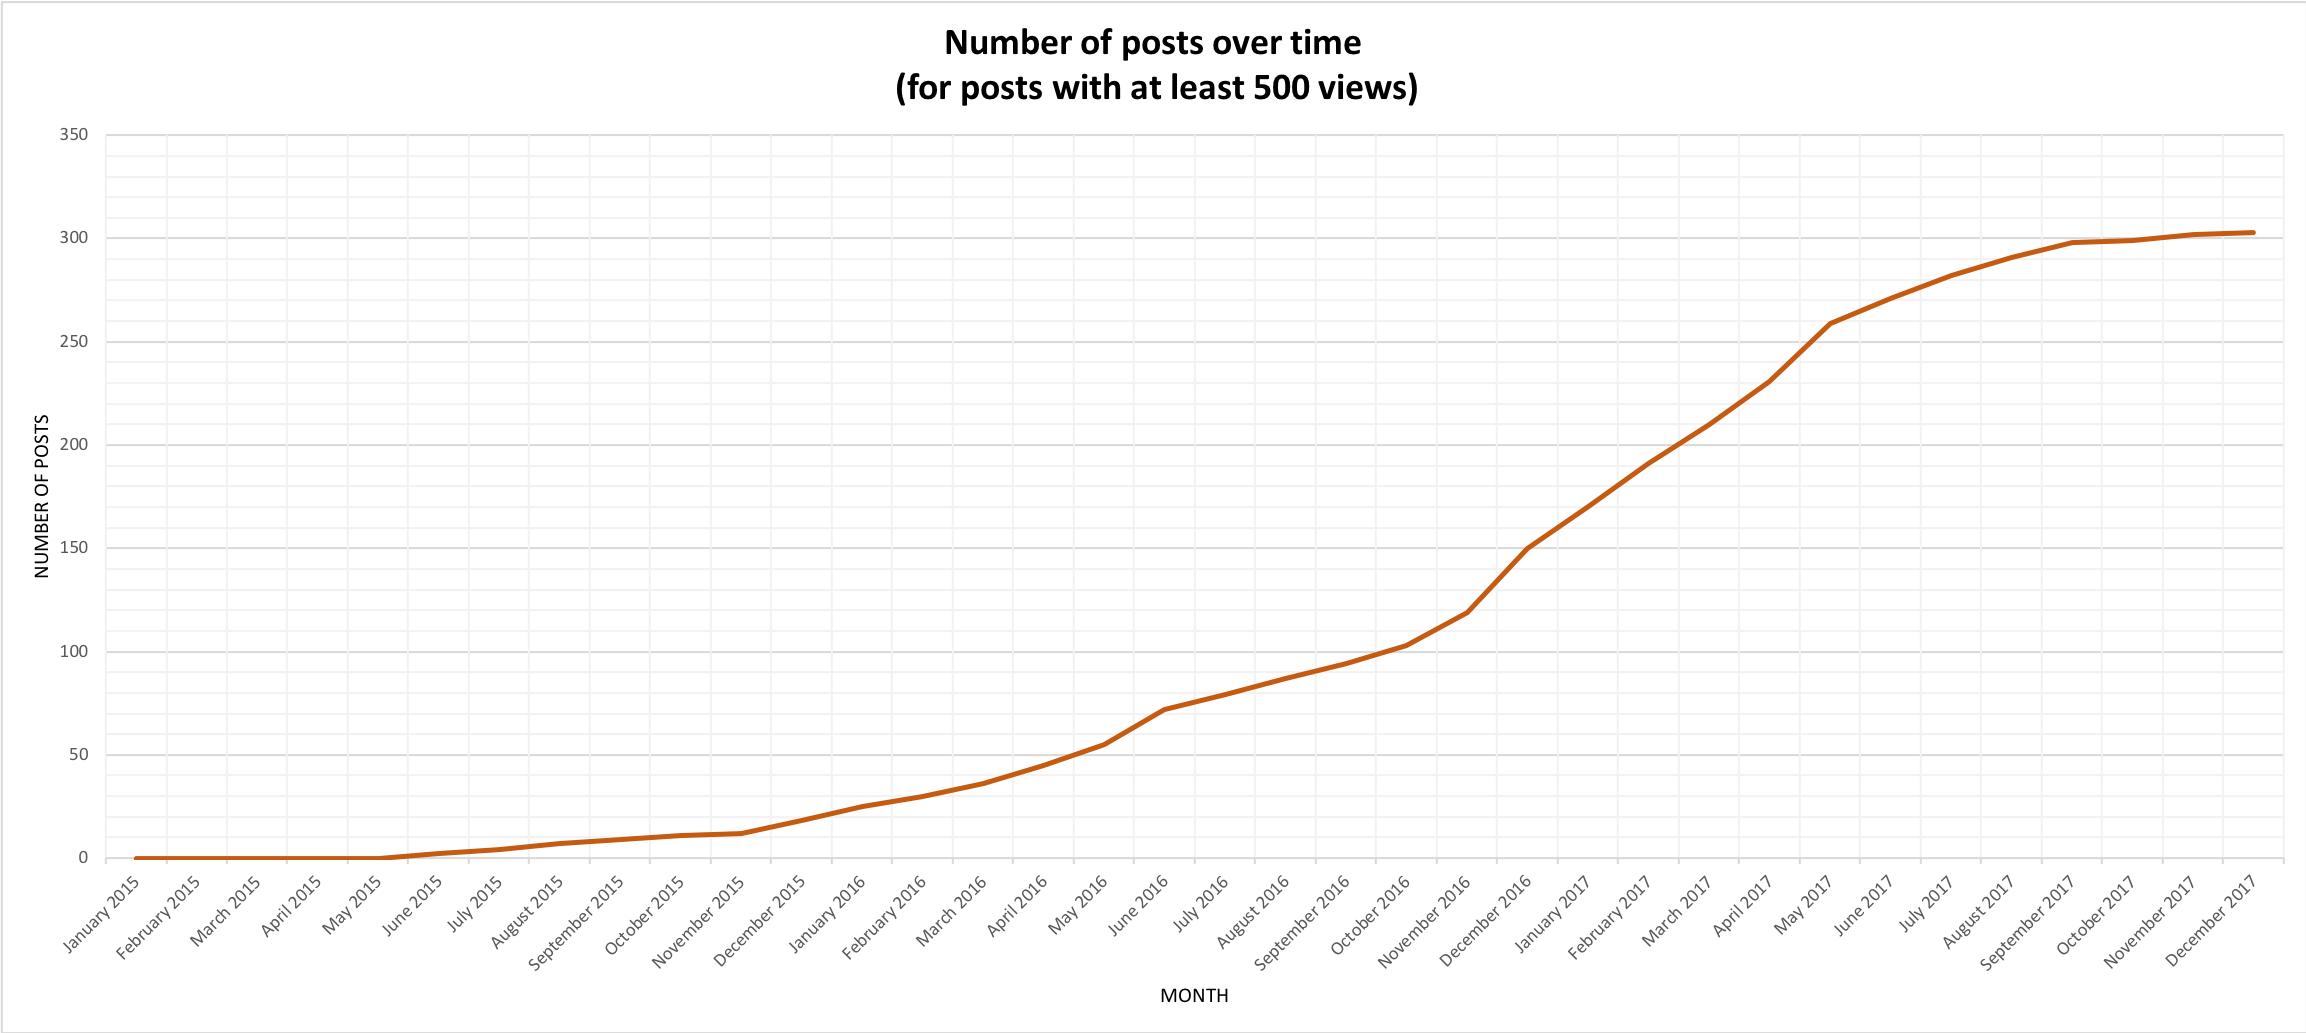
\includegraphics[width=\textwidth,height=\textheight,keepaspectratio]{RQ4-NumPostsOverTime_500Views.png}
    \caption{Growth in the number of posts over time, for posts with at least 500 views}
    \label{fig:3GrowthInNumPosts500Views}
\end{figure}
\begin{figure}[ht]
	\centering
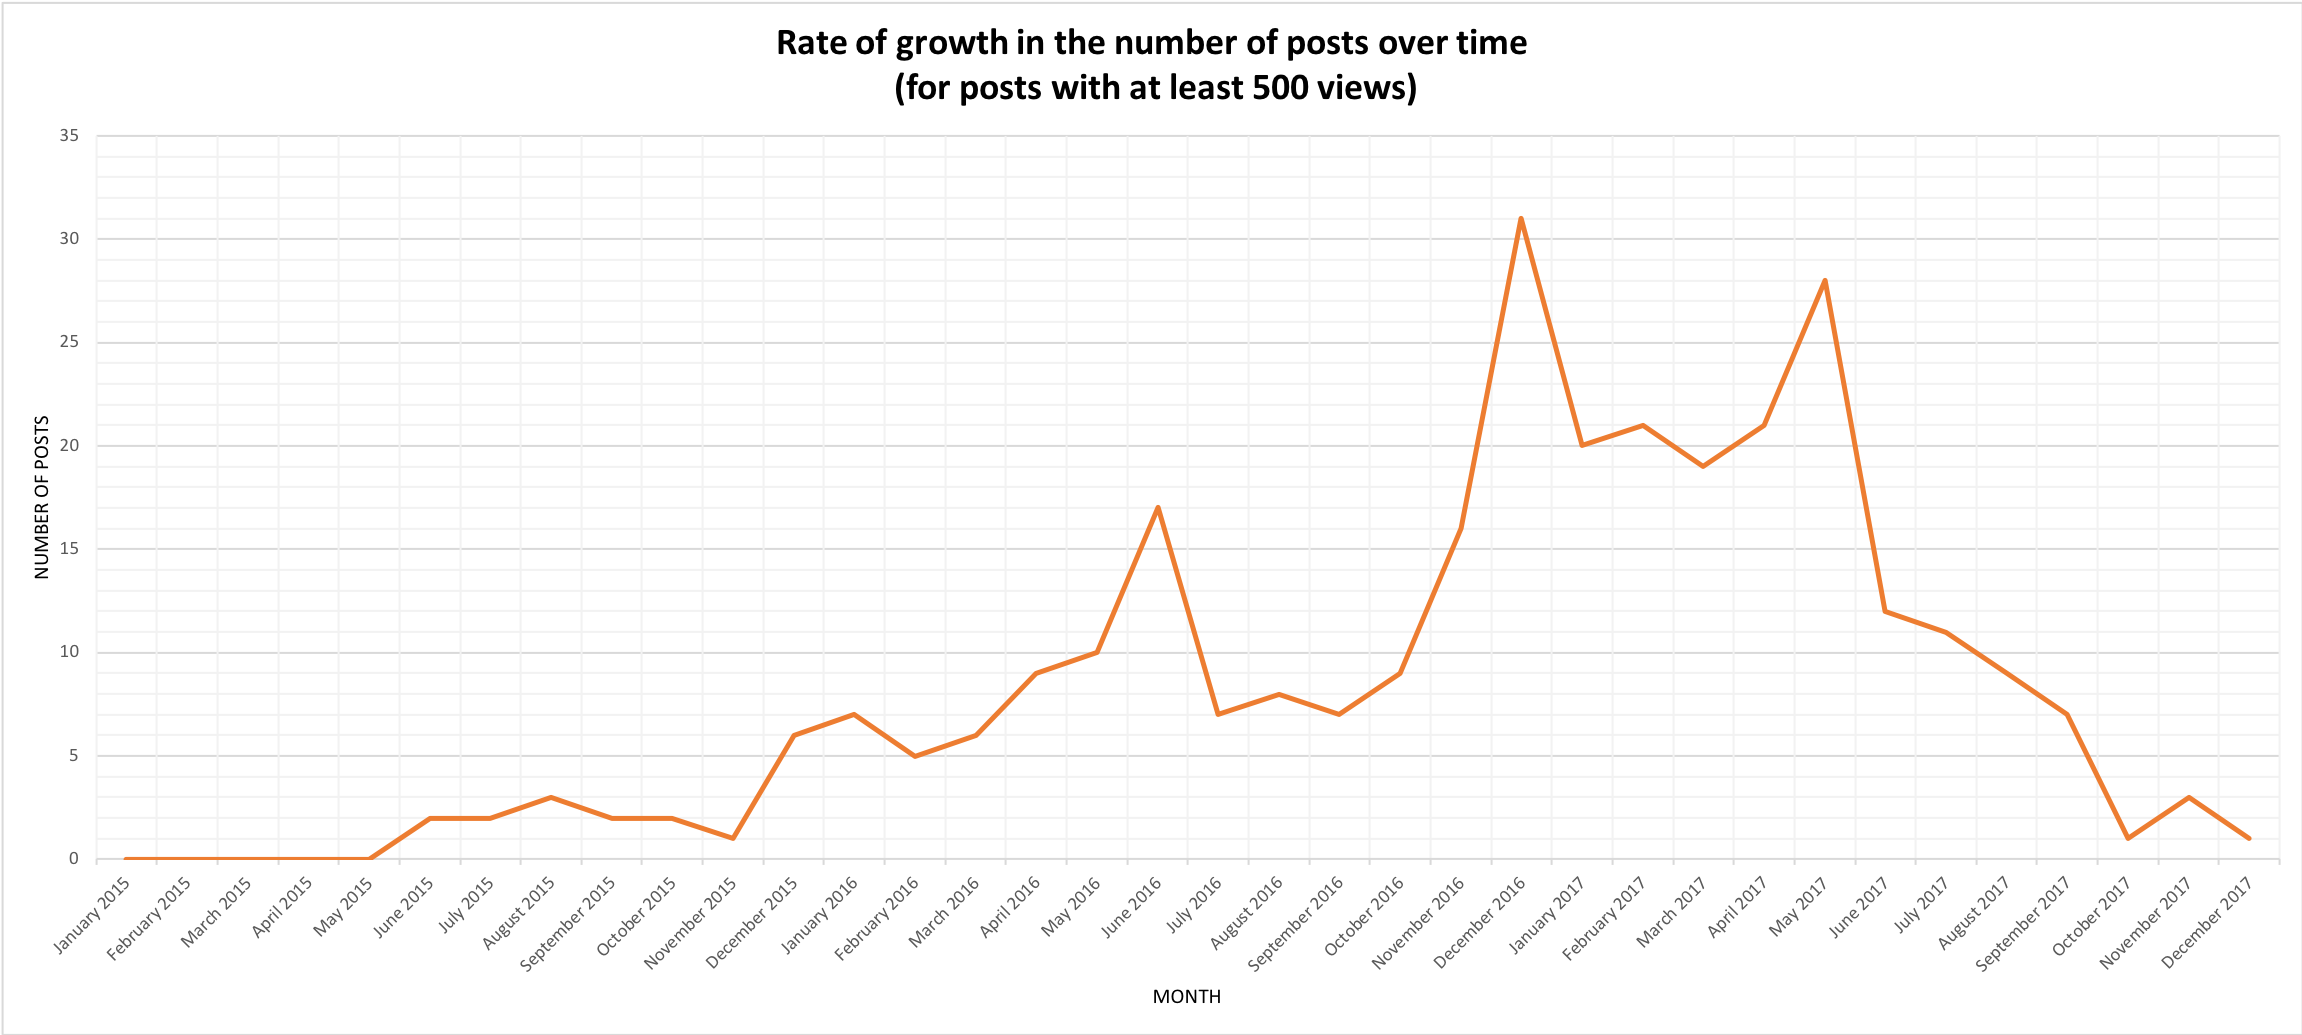
\includegraphics[width=\textwidth,height=\textheight,keepaspectratio]{RQ4-RateNumPostsOverTime_500Views.png}
    \caption{Rate of Growth in the number of posts over time, for posts with at least 500 views}
    \label{fig:3.1RateGrowthInNumPosts500Views}
\end{figure}

\pagebreak
\begin{table}[H] %place tables right after subheading and use H tag to force in under subheading%
\centering
%Resizebox encases the tabular tag to ensure we fit within a column%
\resizebox{\columnwidth}{!}{%
\begin{tabular}{|c|l|c|c|}
\hline
\textbf{Year} & \textbf{Month} & \textbf{Number of New Posts} & \textbf{Cumulative Number of Posts} \\ \hline
\multirow{12}{*}{2015} & January 2015 & 0 & 0 \\ \cline{2-4} 
 & February 2015 & 0 & 0 \\ \cline{2-4} 
 & March 2015 & 0 & 0 \\ \cline{2-4} 
 & April 2015 & 0 & 0 \\ \cline{2-4} 
 & May 2015 & 1 & 1 \\ \cline{2-4} 
 & June 2015 & 2 & 3 \\ \cline{2-4} 
 & July 2015 & 2 & 5 \\ \cline{2-4} 
 & August 2015 & 3 & 8 \\ \cline{2-4} 
 & September 2015 & 2 & 10 \\ \cline{2-4} 
 & October 2015 & 2 & 12 \\ \cline{2-4} 
 & November 2015 & 2 & 14 \\ \cline{2-4} 
 & December 2015 & 8 & 22 \\ \hline
\multirow{12}{*}{2016} & January 2016 & 8 & 30 \\ \cline{2-4} 
 & February 2016 & 7 & 37 \\ \cline{2-4} 
 & March 2016 & 11 & 48 \\ \cline{2-4} 
 & April 2016 & 14 & 62 \\ \cline{2-4} 
 & May 2016 & 22 & 84 \\ \cline{2-4} 
 & June 2016 & 29 & 113 \\ \cline{2-4} 
 & July 2016 & 23 & 136 \\ \cline{2-4} 
 & August 2016 & 23 & 159 \\ \cline{2-4} 
 & September 2016 & 20 & 179 \\ \cline{2-4} 
 & October 2016 & 18 & 197 \\ \cline{2-4} 
 & November 2016 & 37 & 234 \\ \cline{2-4} 
 & December 2016 & 69 & 303 \\ \hline
\multirow{12}{*}{2017} & January 2017 & 76 & 379 \\ \cline{2-4} 
 & February 2017 & 65 & 444 \\ \cline{2-4} 
 & March 2017 & 66 & 510 \\ \cline{2-4} 
 & April 2017 & 77 & 587 \\ \cline{2-4} 
 & May 2017 & 131 & 718 \\ \cline{2-4} 
 & June 2017 & 120 & 838 \\ \cline{2-4} 
 & July 2017 & 150 & 988 \\ \cline{2-4} 
 & August 2017 & 132 & 1120 \\ \cline{2-4} 
 & September 2017 & 107 & 1227 \\ \cline{2-4} 
 & October 2017 & 132 & 1359 \\ \cline{2-4} 
 & November 2017 & 177 & 1536 \\ \cline{2-4} 
 & December 2017 & 164 & 1700 \\ \hline
\multirow{3}{*}{2018} & January 2018 & 164 & 1864 \\ \cline{2-4} 
 & February 2018 & 178 & 2042 \\ \cline{2-4} 
 & March 2018 & 67 & 2109 \\ \hline
\end{tabular}
}
\caption{Monthly growth rate and sum of posts at end of specific month, regardless of post viewcount}
\label{table:GrowthRateAndGrowthAllViews}
\end{table}
\pagebreak

\begin{figure}[ht]
	\centering
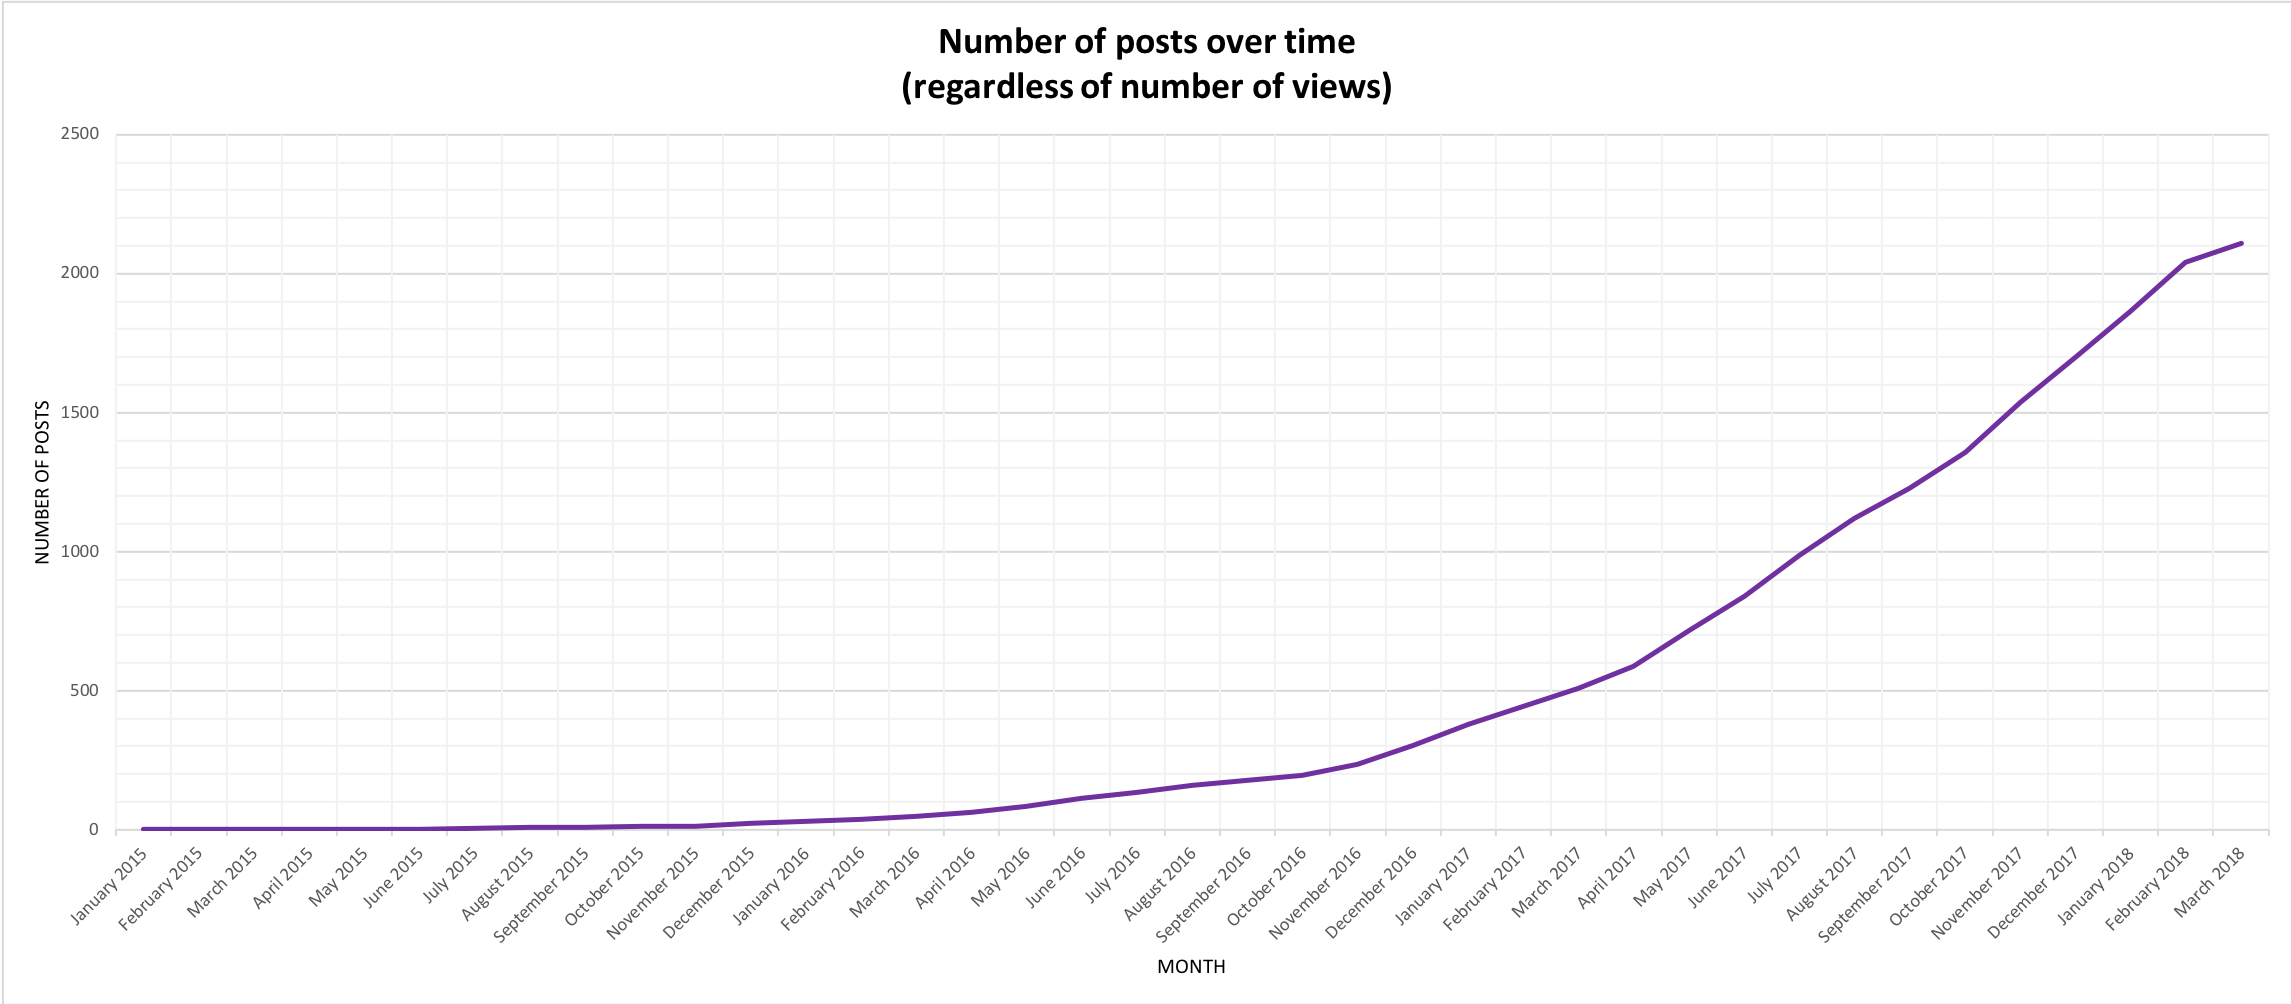
\includegraphics[width=\textwidth,height=\textheight,keepaspectratio]{RQ4-NumPostsOverTime_AllViews.png}
    \caption{Growth in the number of posts over time, regardless of number of views}
    \label{fig:4GrowthInNumPostsAllViews}
\end{figure}
\begin{figure}[ht]
	\centering
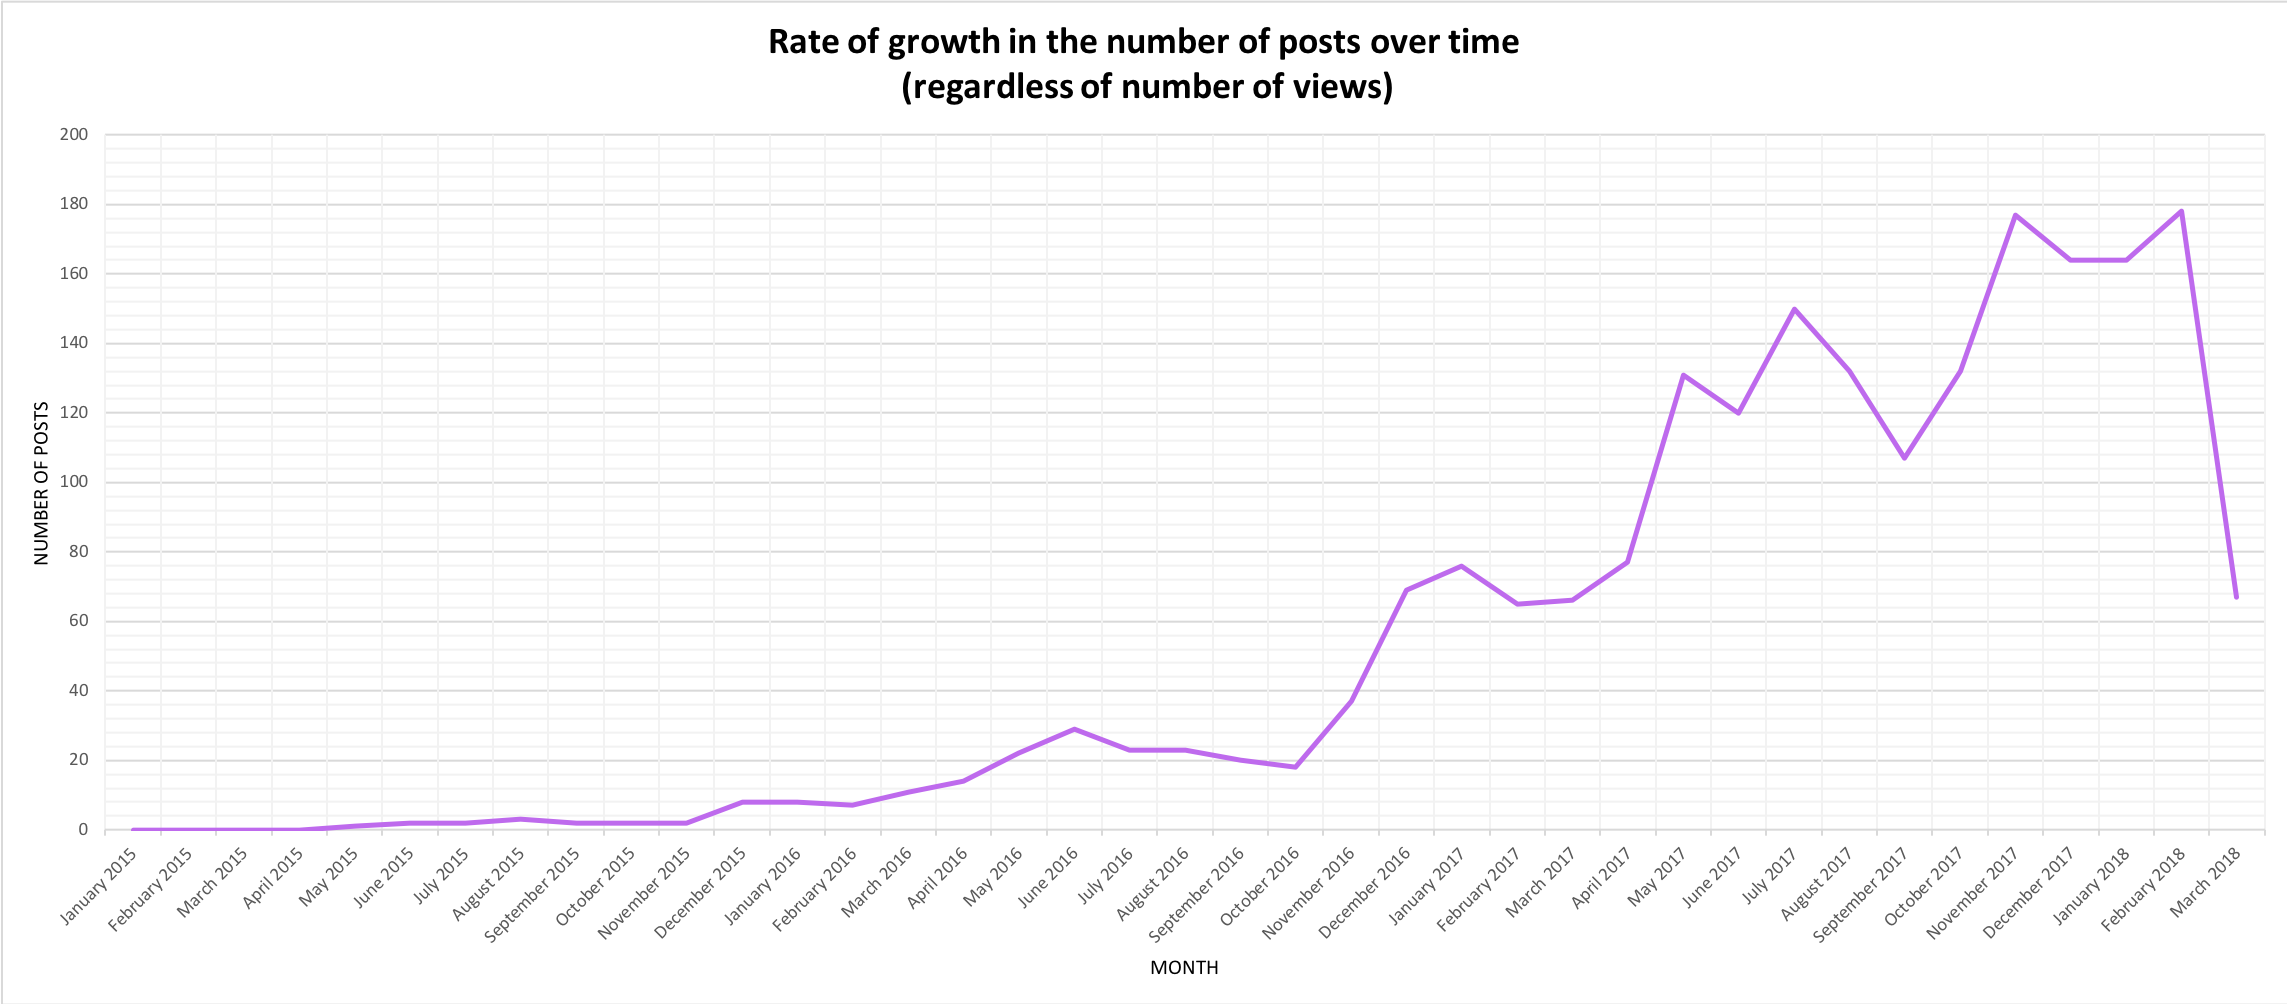
\includegraphics[width=\textwidth,height=\textheight,keepaspectratio]{RQ4-RateNumPostsOverTime_AllViews.png}
    \caption{Rate of Growth in the number of posts over time, regardless of number of views}
    \label{fig:4.1RateGrowthInNumPostsAllViews}
\end{figure}

\begin{figure}[ht]
	\centering
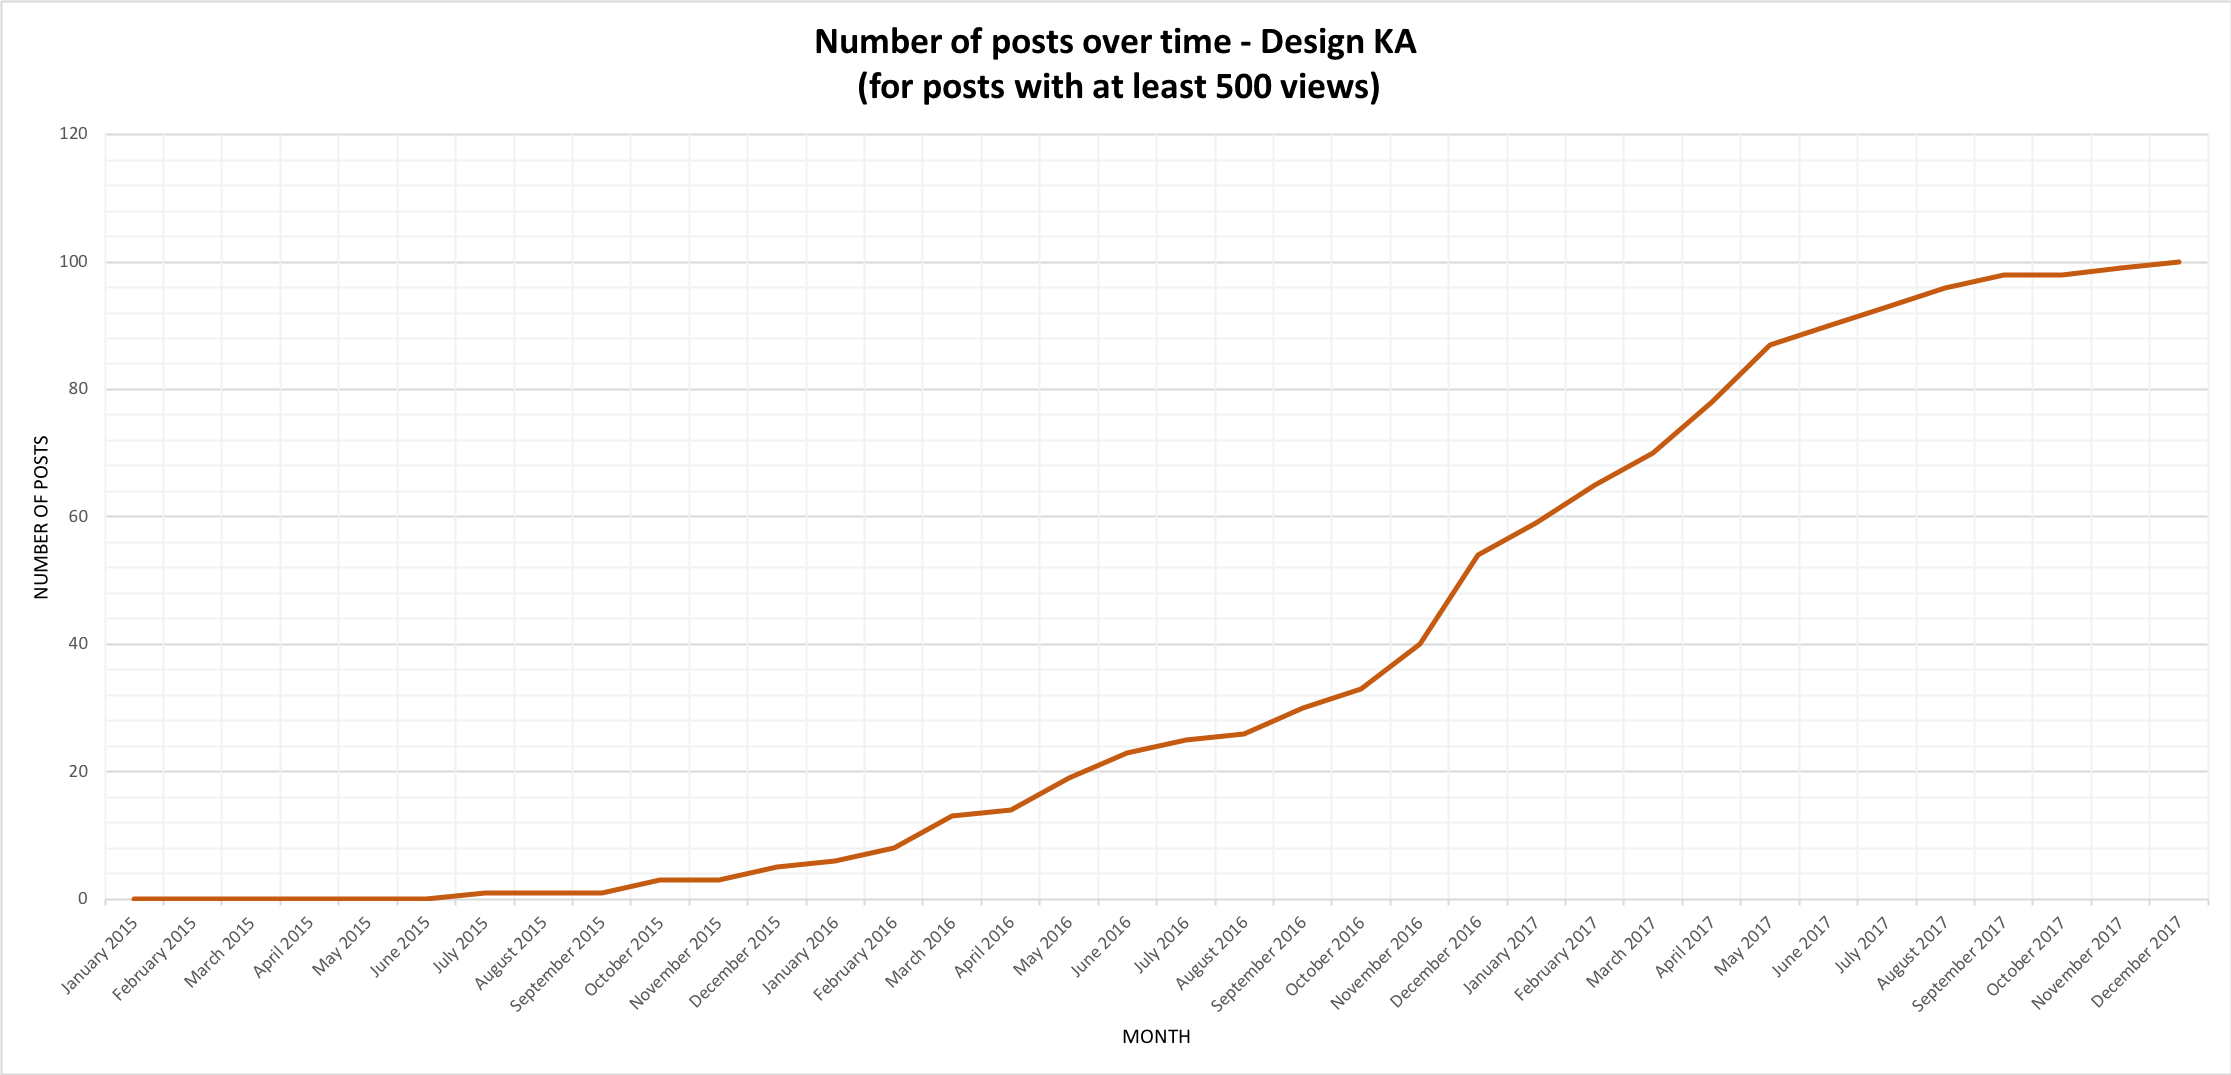
\includegraphics[width=\textwidth,height=\textheight,keepaspectratio]{RQ5-DesignNumPostsOverTime_500Views.png}
    \caption{Growth in the number of posts over time for Design KA, based on posts with at least 500 views}
    \label{fig:5DesignGrowthInNumPosts500Views}
\end{figure}
\begin{figure}[ht]
	\centering
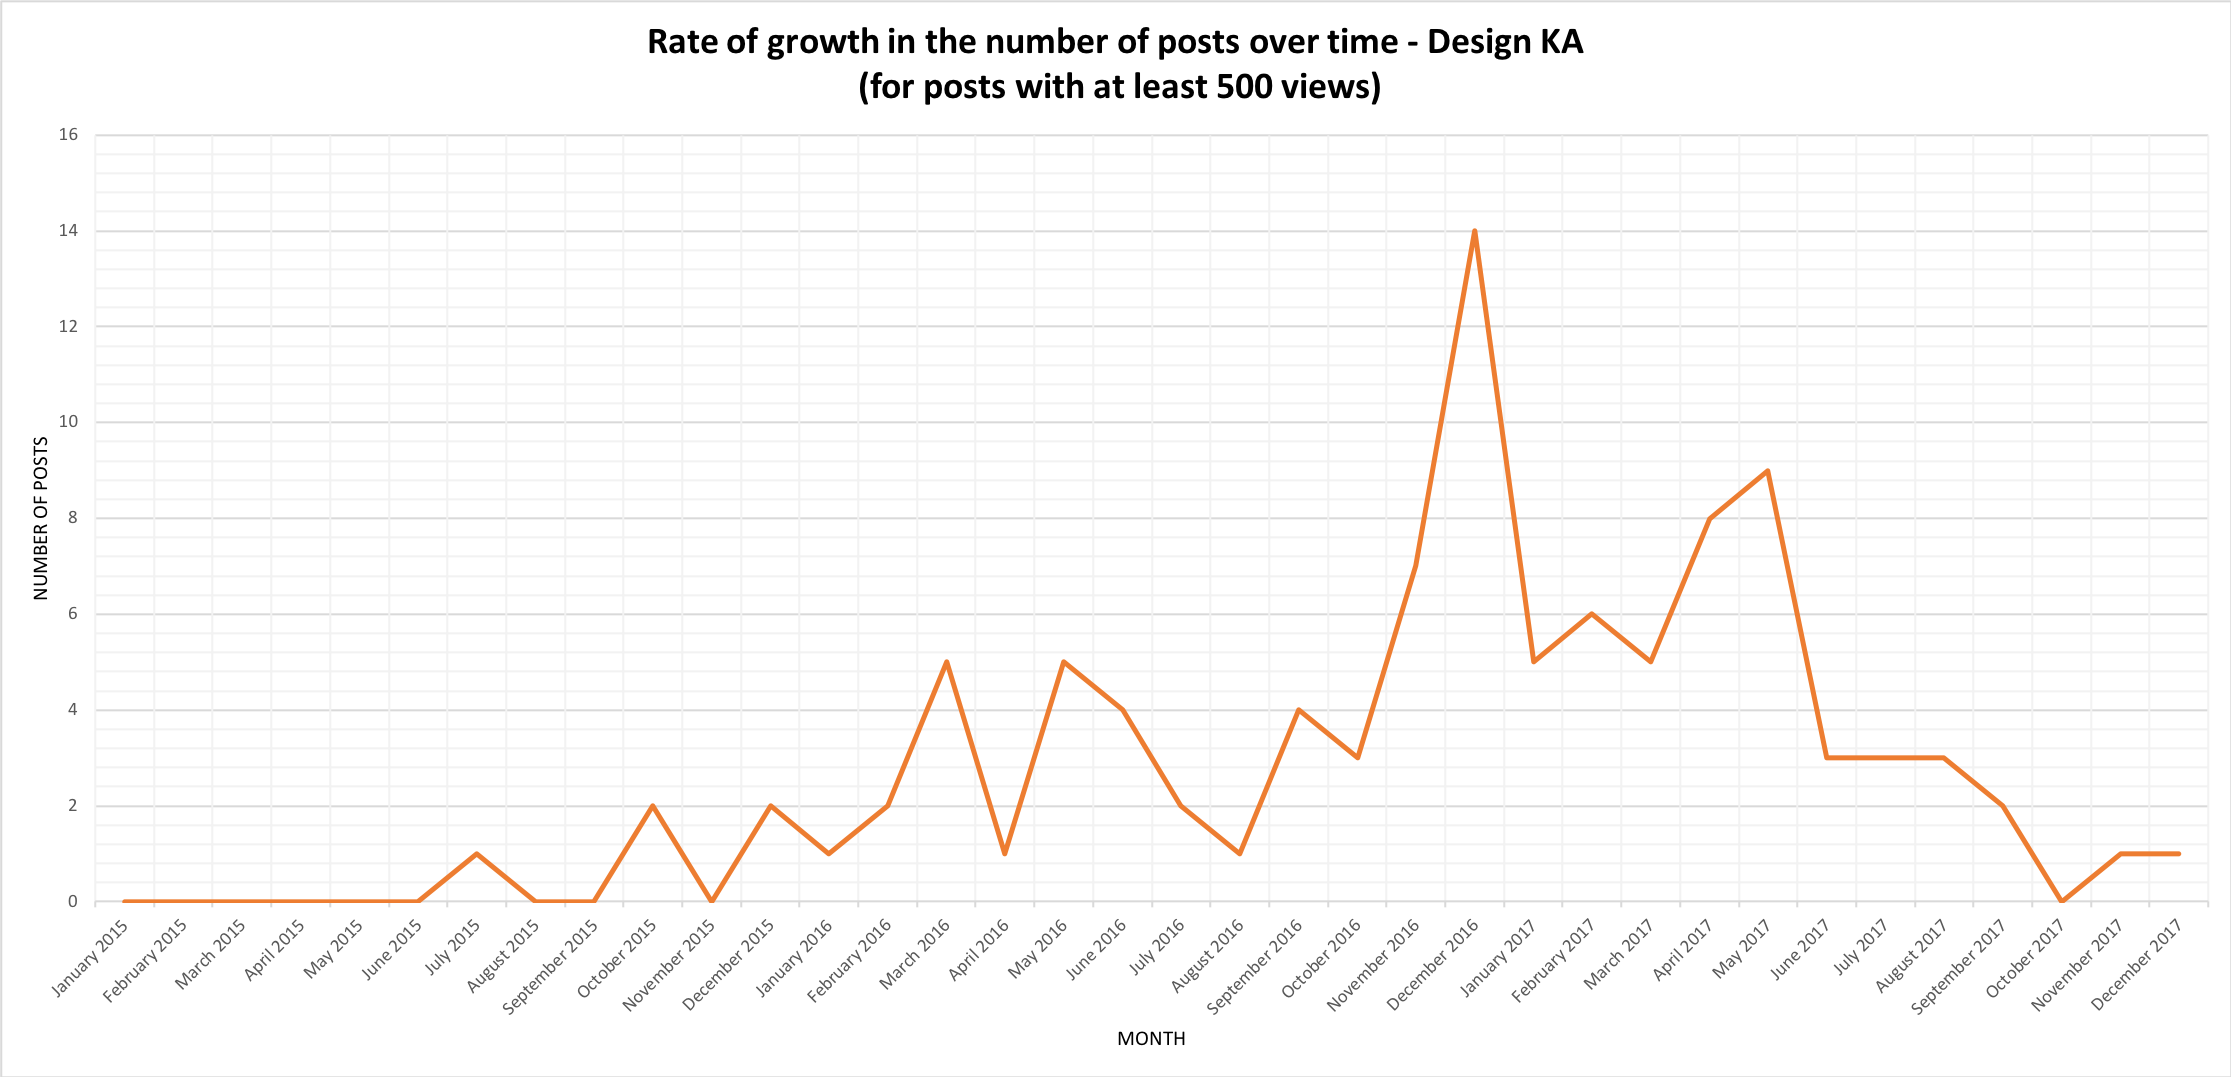
\includegraphics[width=\textwidth,height=\textheight,keepaspectratio]{RQ5-DesignRateNumPostsOverTime_500Views.png}
    \caption{Rate of Growth in the number of posts over time for Design KA, based on posts with at least 500 views}
    \label{fig:5.1DesignRateGrowthInNumPosts500Views}
\end{figure}

\begin{figure}[ht]
	\centering
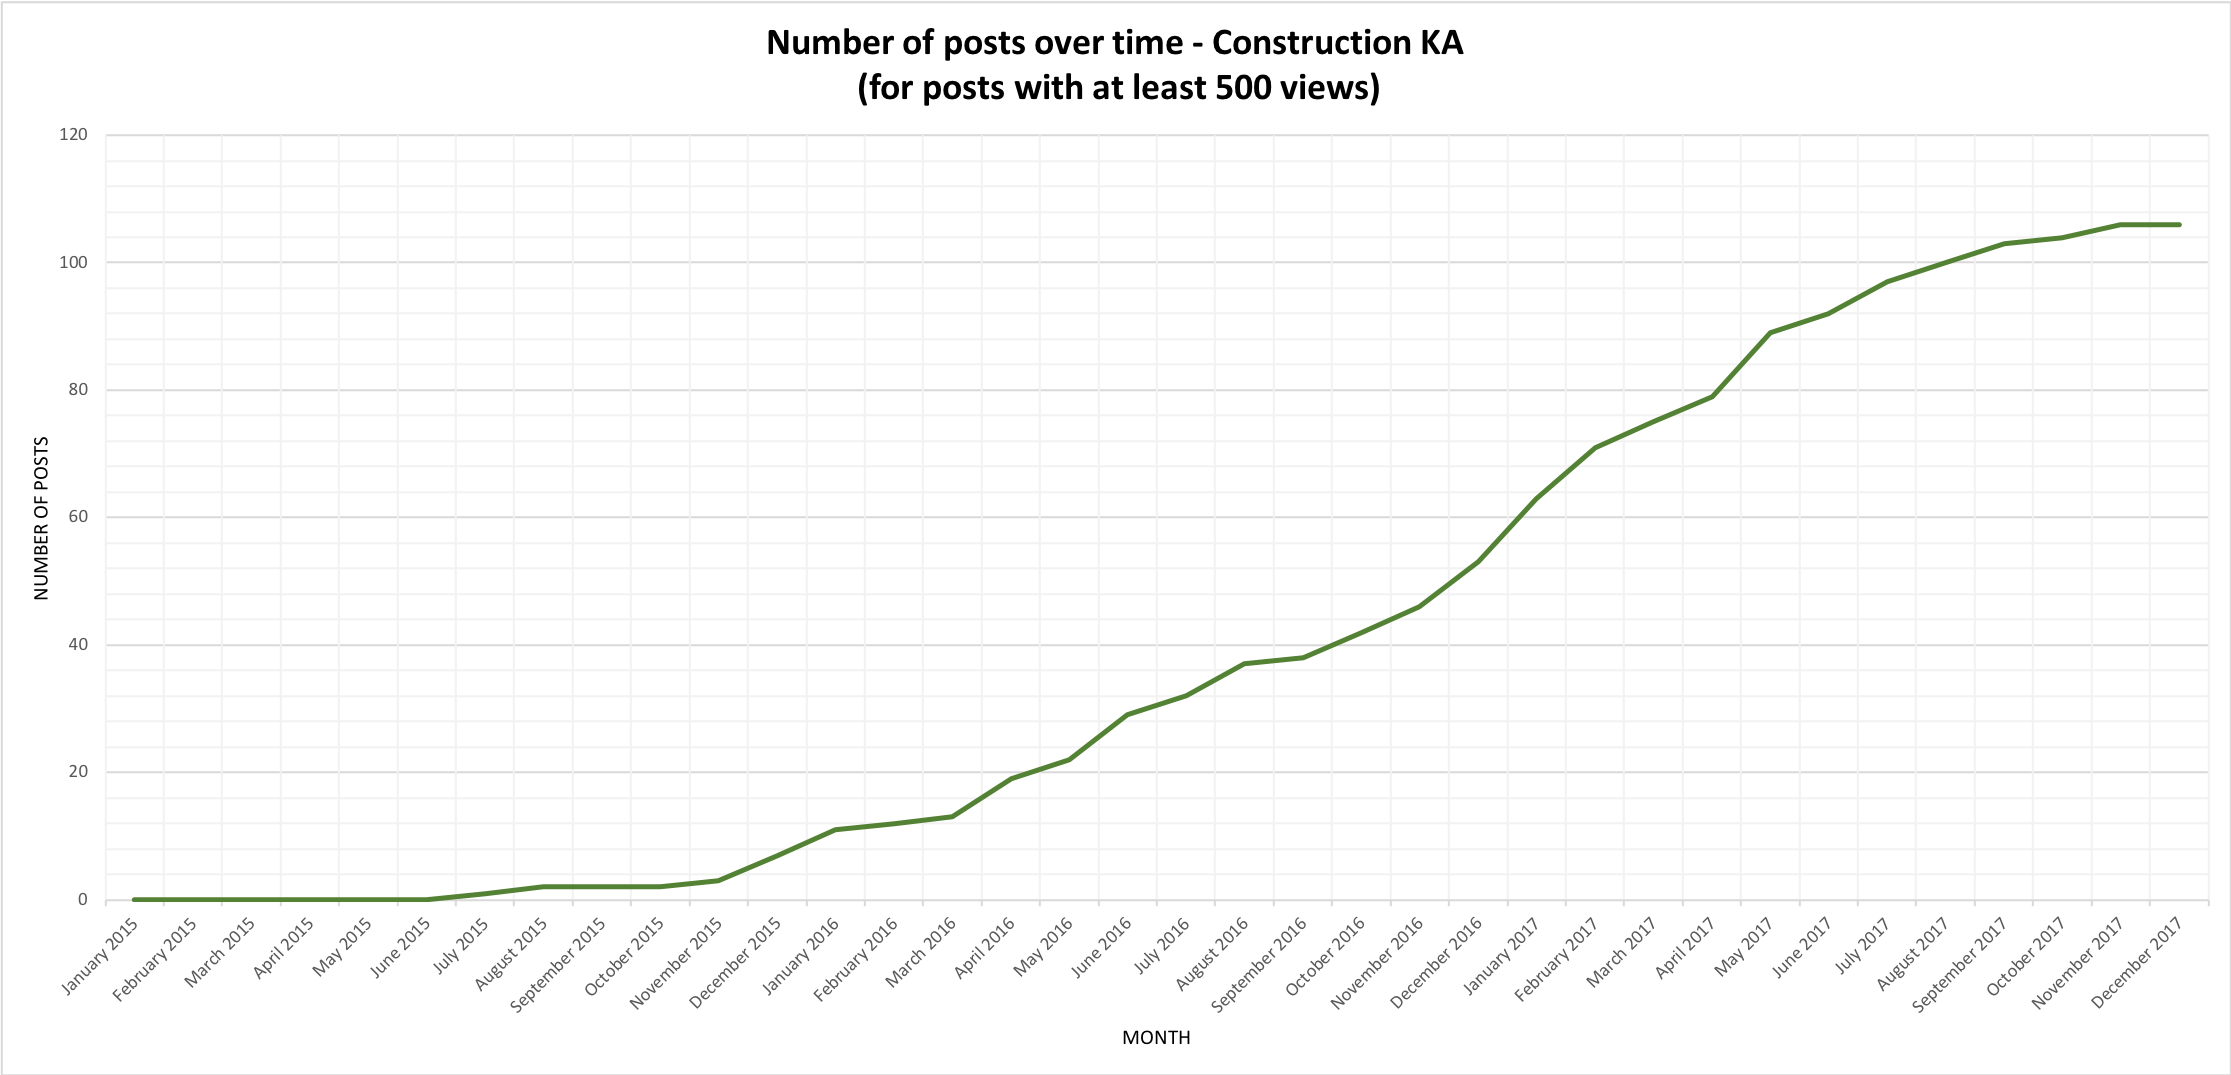
\includegraphics[width=\textwidth,height=\textheight,keepaspectratio]{RQ5-ConstructionNumPostsOverTime_500Views.png}
    \caption{Growth in the number of posts over time for Construction KA, based on posts with at least 500 views}
    \label{fig:6ConstructionGrowthInNumPosts500Views}
\end{figure}
\begin{figure}[ht]
	\centering
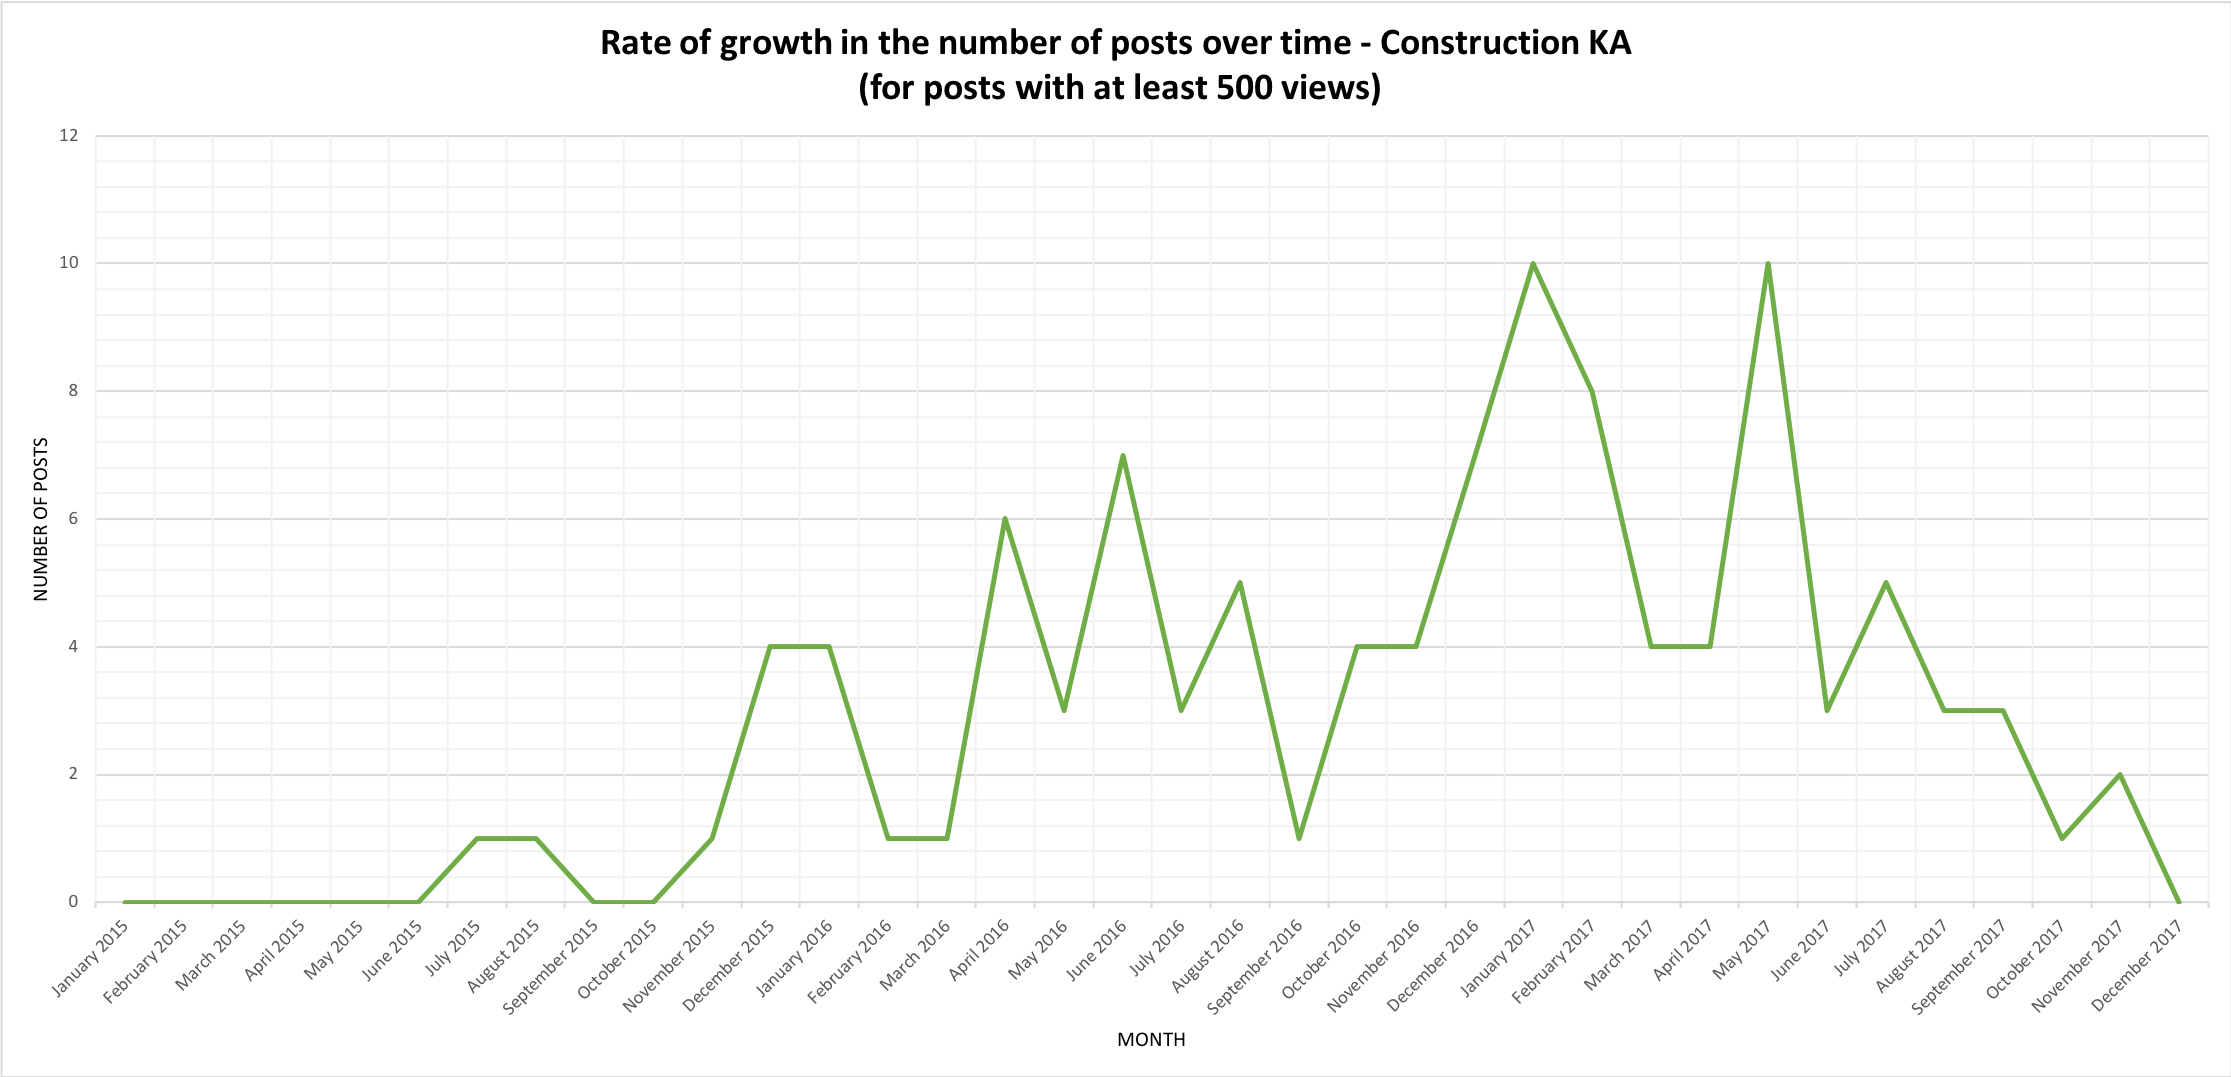
\includegraphics[width=\textwidth,height=\textheight,keepaspectratio]{RQ5-ConstructionRateNumPostsOverTime_500Views.png}
    \caption{Rate of Growth in the number of posts over time for Construction KA, based on posts with at least 500 views}
    \label{fig:6.1ConstructionRateGrowthInNumPosts500Views}
\end{figure}

\begin{figure}[ht]
	\centering
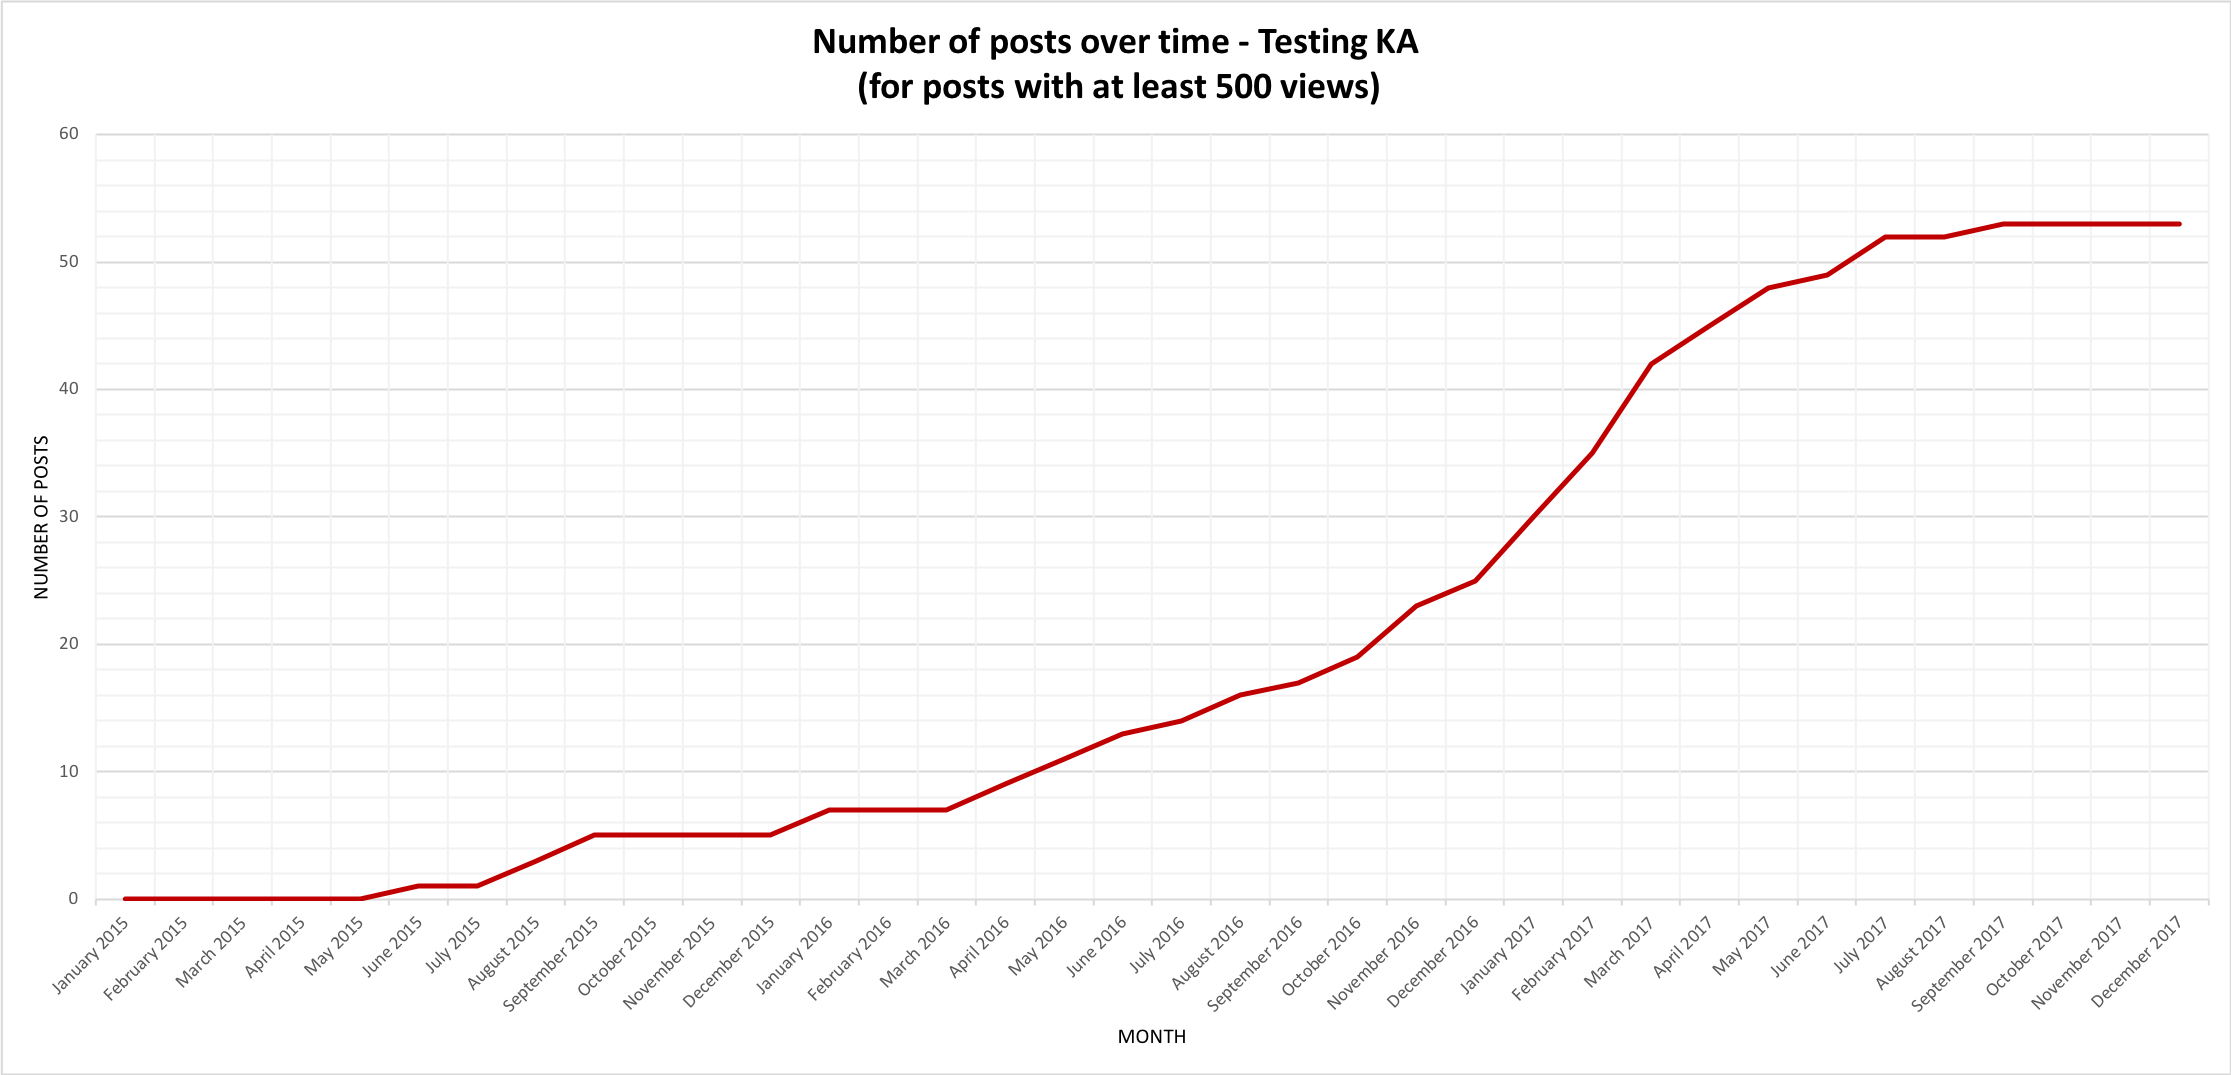
\includegraphics[width=\textwidth,height=\textheight,keepaspectratio]{RQ5-TestingNumPostsOverTime_500Views.png}
    \caption{Growth in the number of posts over time for Testing KA, based on posts with at least 500 views}
    \label{fig:7TestingGrowthInNumPosts500Views}
\end{figure}
\begin{figure}[ht]
	\centering
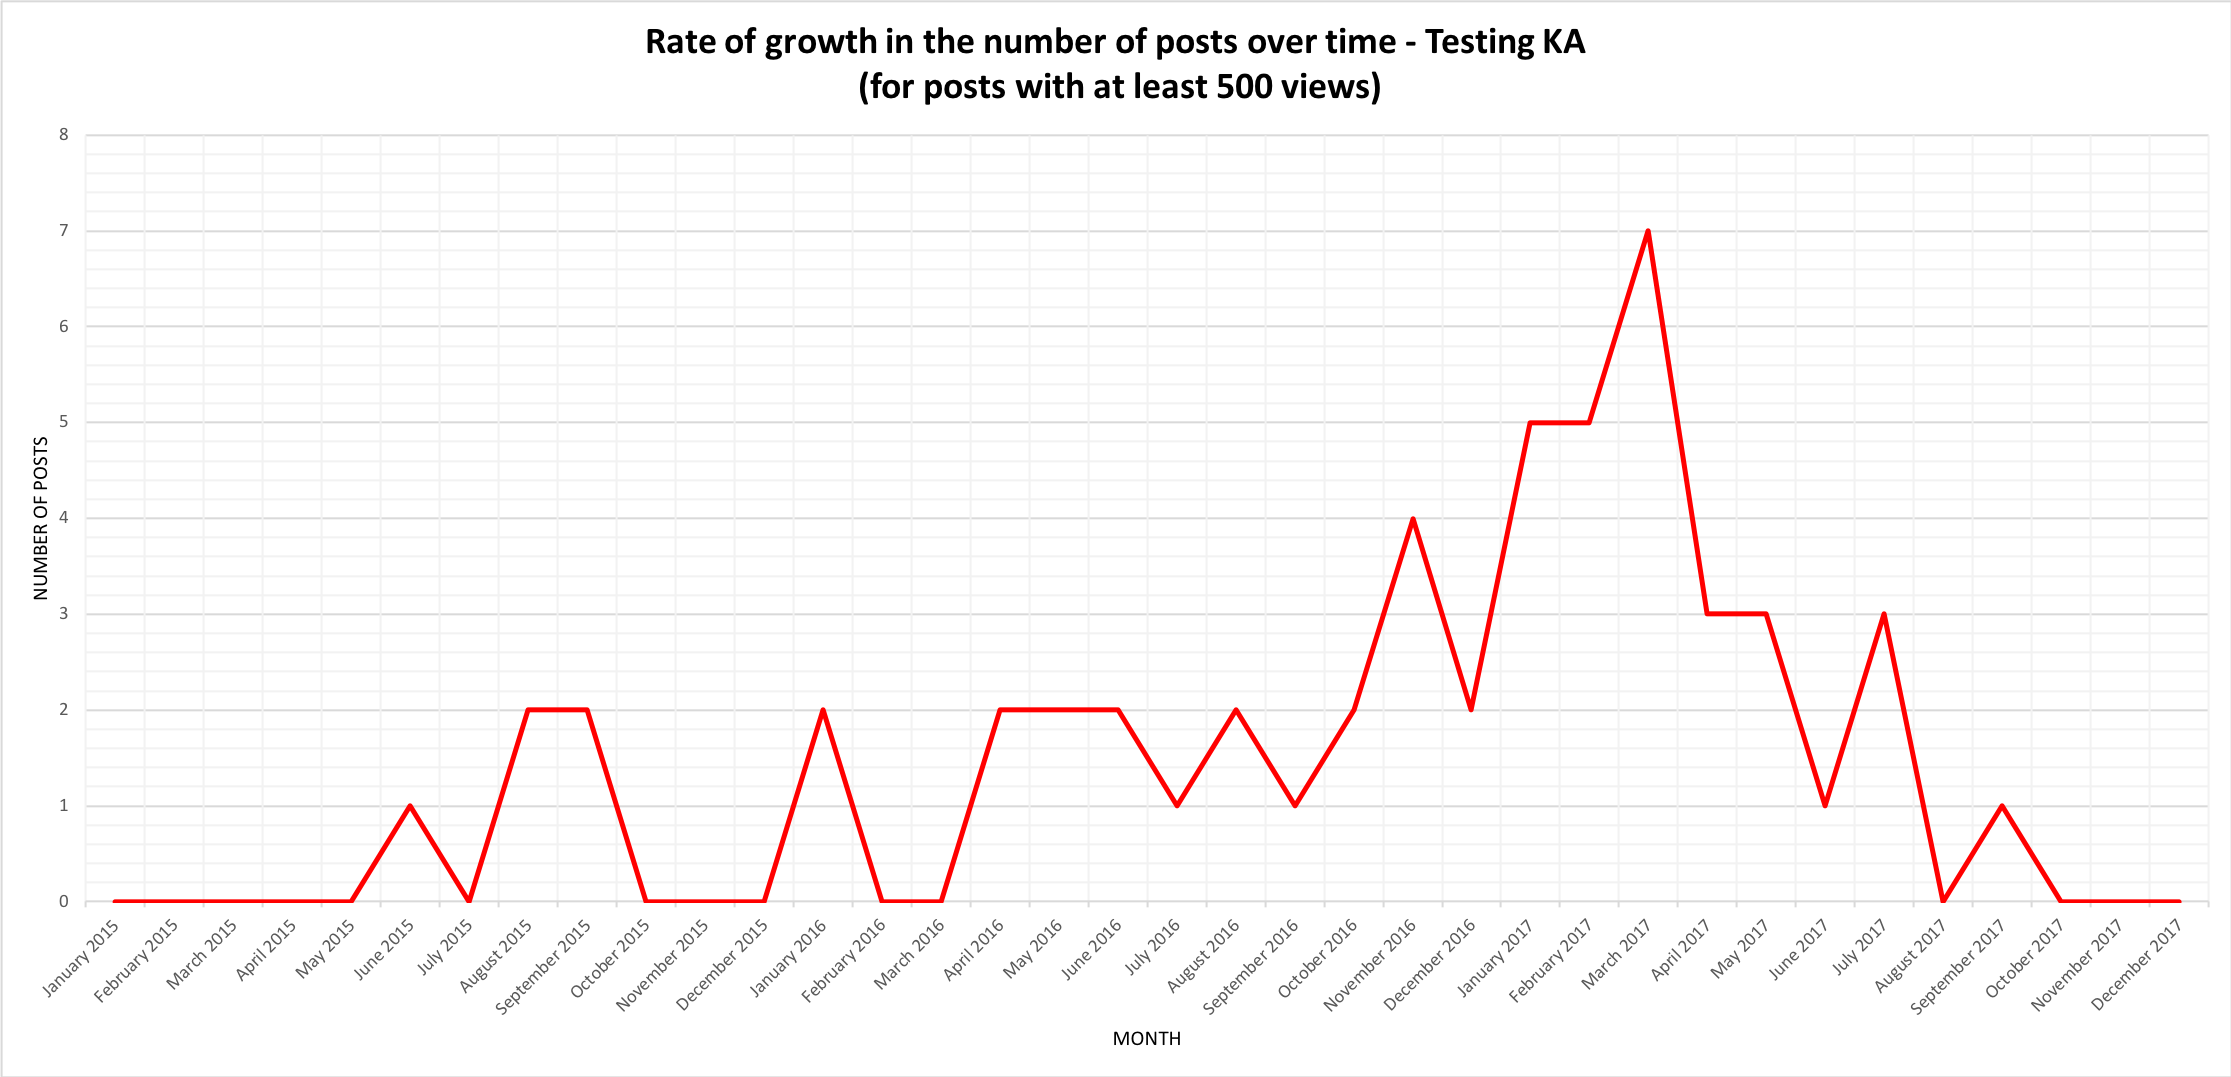
\includegraphics[width=\textwidth,height=\textheight,keepaspectratio]{RQ5-TestingRateNumPostsOverTime_500Views.png}
    \caption{Rate of Growth in the number of posts over time for Testing KA, based on posts with at least 500 views}
    \label{fig:7.1TestingRateGrowthInNumPosts500Views}
\end{figure}


\begin{figure}[ht]
	\centering
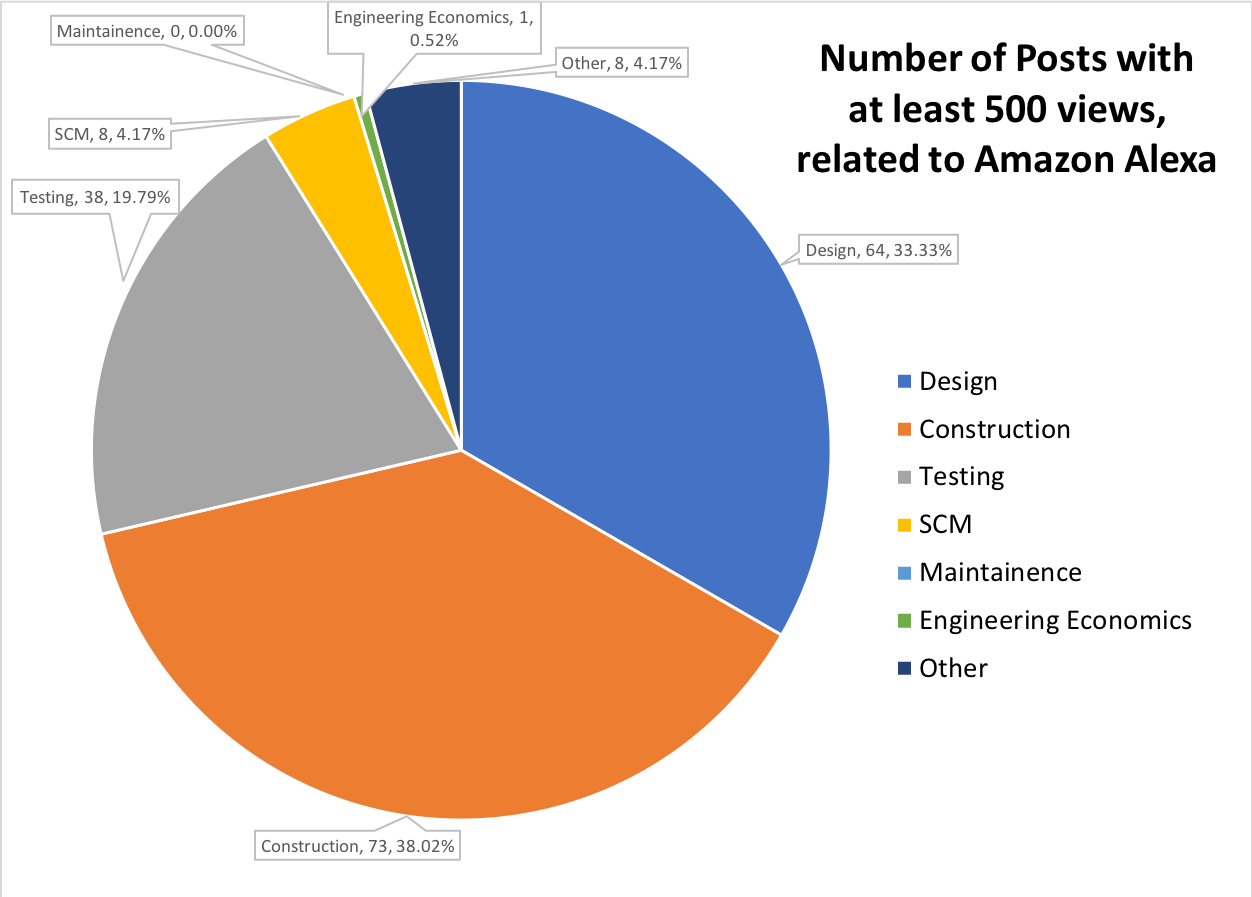
\includegraphics[width=0.7\textwidth,height=0.7\textheight,keepaspectratio]{RQ6_AlexaPosts500.png}
    \caption{All Alexa related posts according to different SWEBOK KAs}
    \label{fig:AlexaPostsSWEBOK}
\end{figure}
\begin{figure}[ht]
	\centering
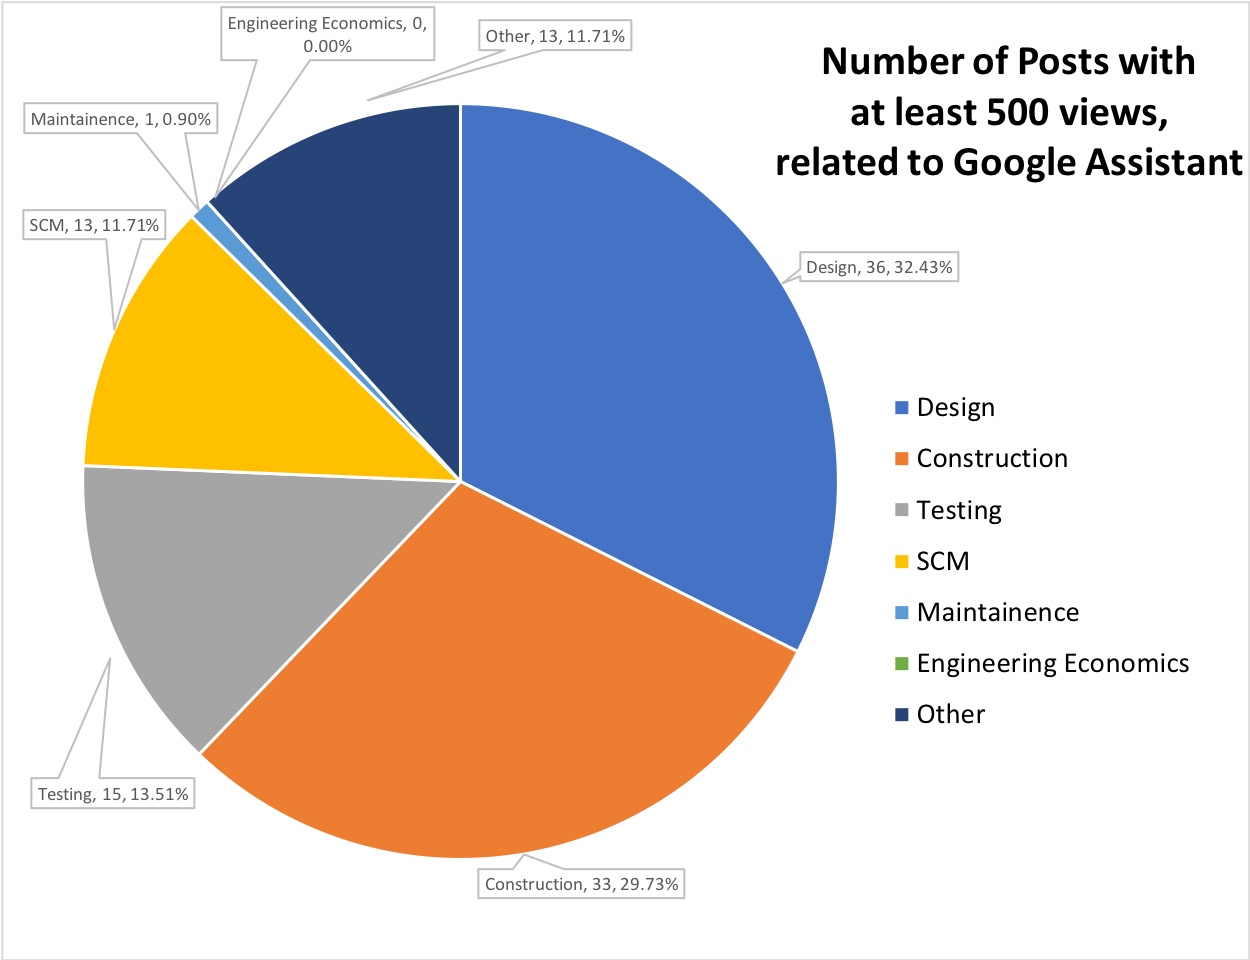
\includegraphics[width=0.7\textwidth,height=0.7\textheight,keepaspectratio]{RQ6_GHomePosts500.png}
    \caption{All Google Assistant related posts according to different SWEBOK KAs}
    \label{fig:GAPostsSwebok}
\end{figure}

\begin{figure}[ht]
	\centering
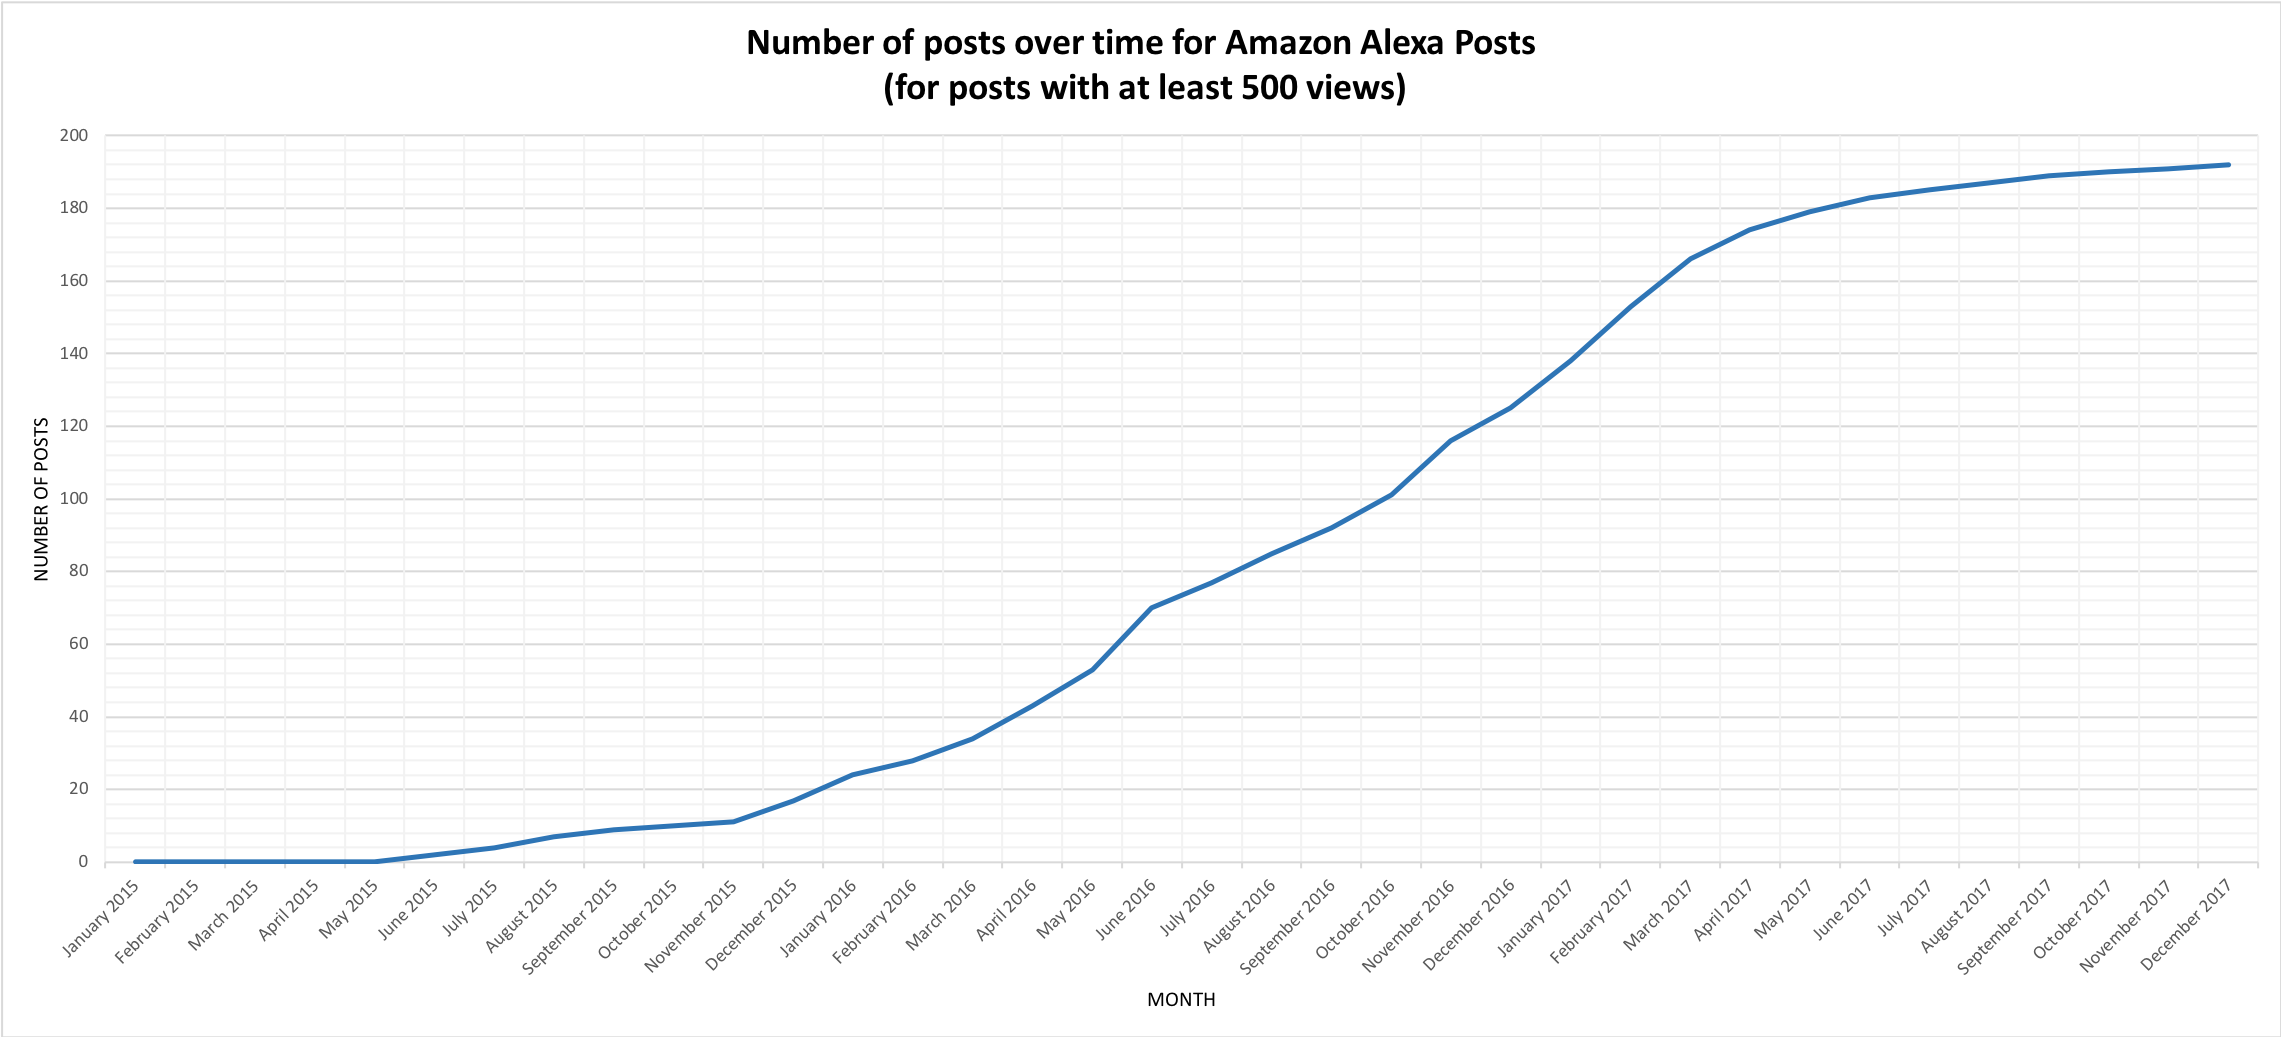
\includegraphics[width=\textwidth,height=\textheight,keepaspectratio]{RQ6-AmazonNumPostsOverTime_500Views.png}
    \caption{Growth in the number of posts over time for posts on Amazon Alexa, based on posts with at least 500 views}
    \label{fig:8AmazonGrowthInNumPosts500Views}
\end{figure}
\begin{figure}[ht]
	\centering
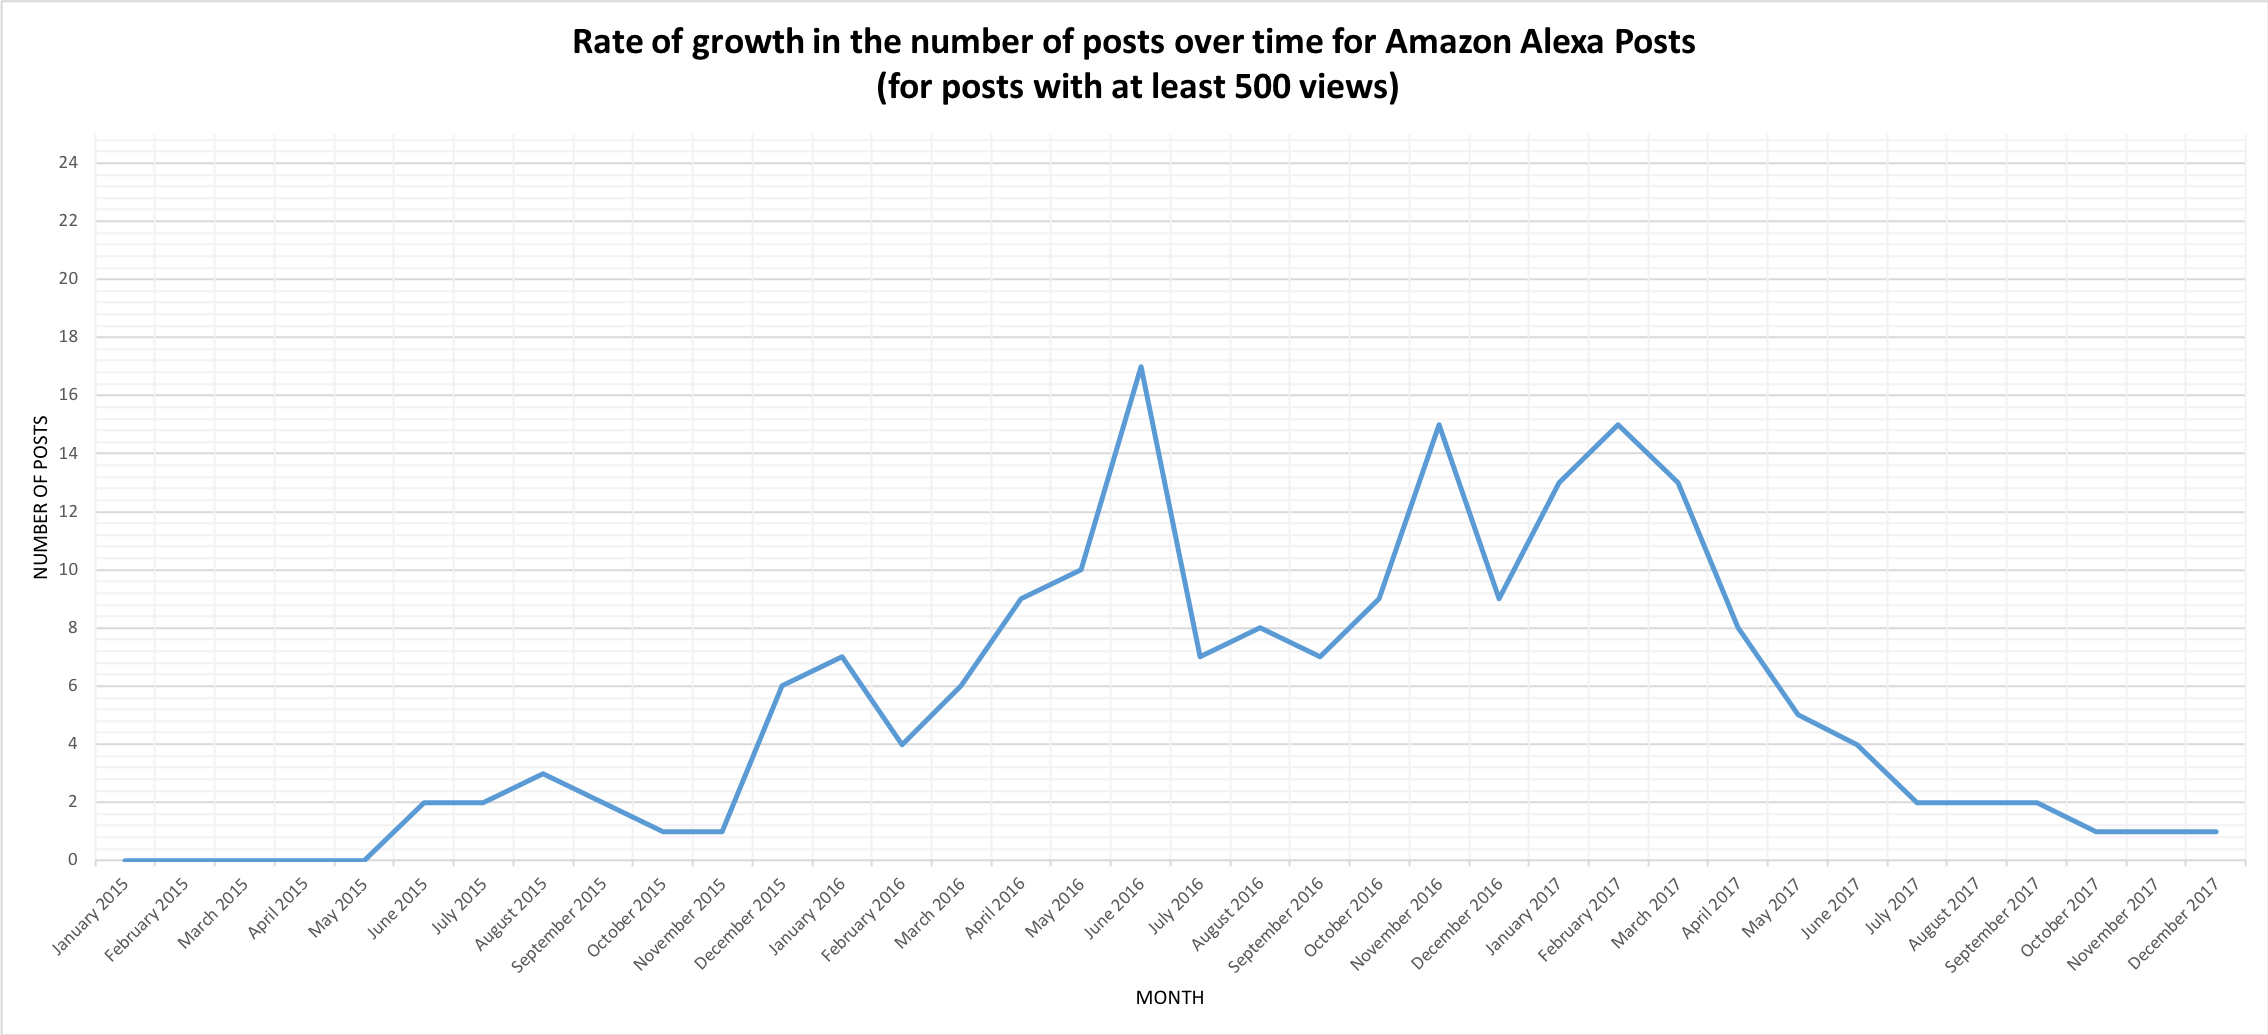
\includegraphics[width=\textwidth,height=\textheight,keepaspectratio]{RQ6-AmazonRateNumPostsOverTime_500Views.png}
    \caption{Rate of Growth in the number of posts over time for posts on Amazon Alexa, based on posts with at least 500 views}
    \label{fig:8.1AmazonRateGrowthInNumPosts500Views}
\end{figure}

\begin{figure}[ht]
	\centering
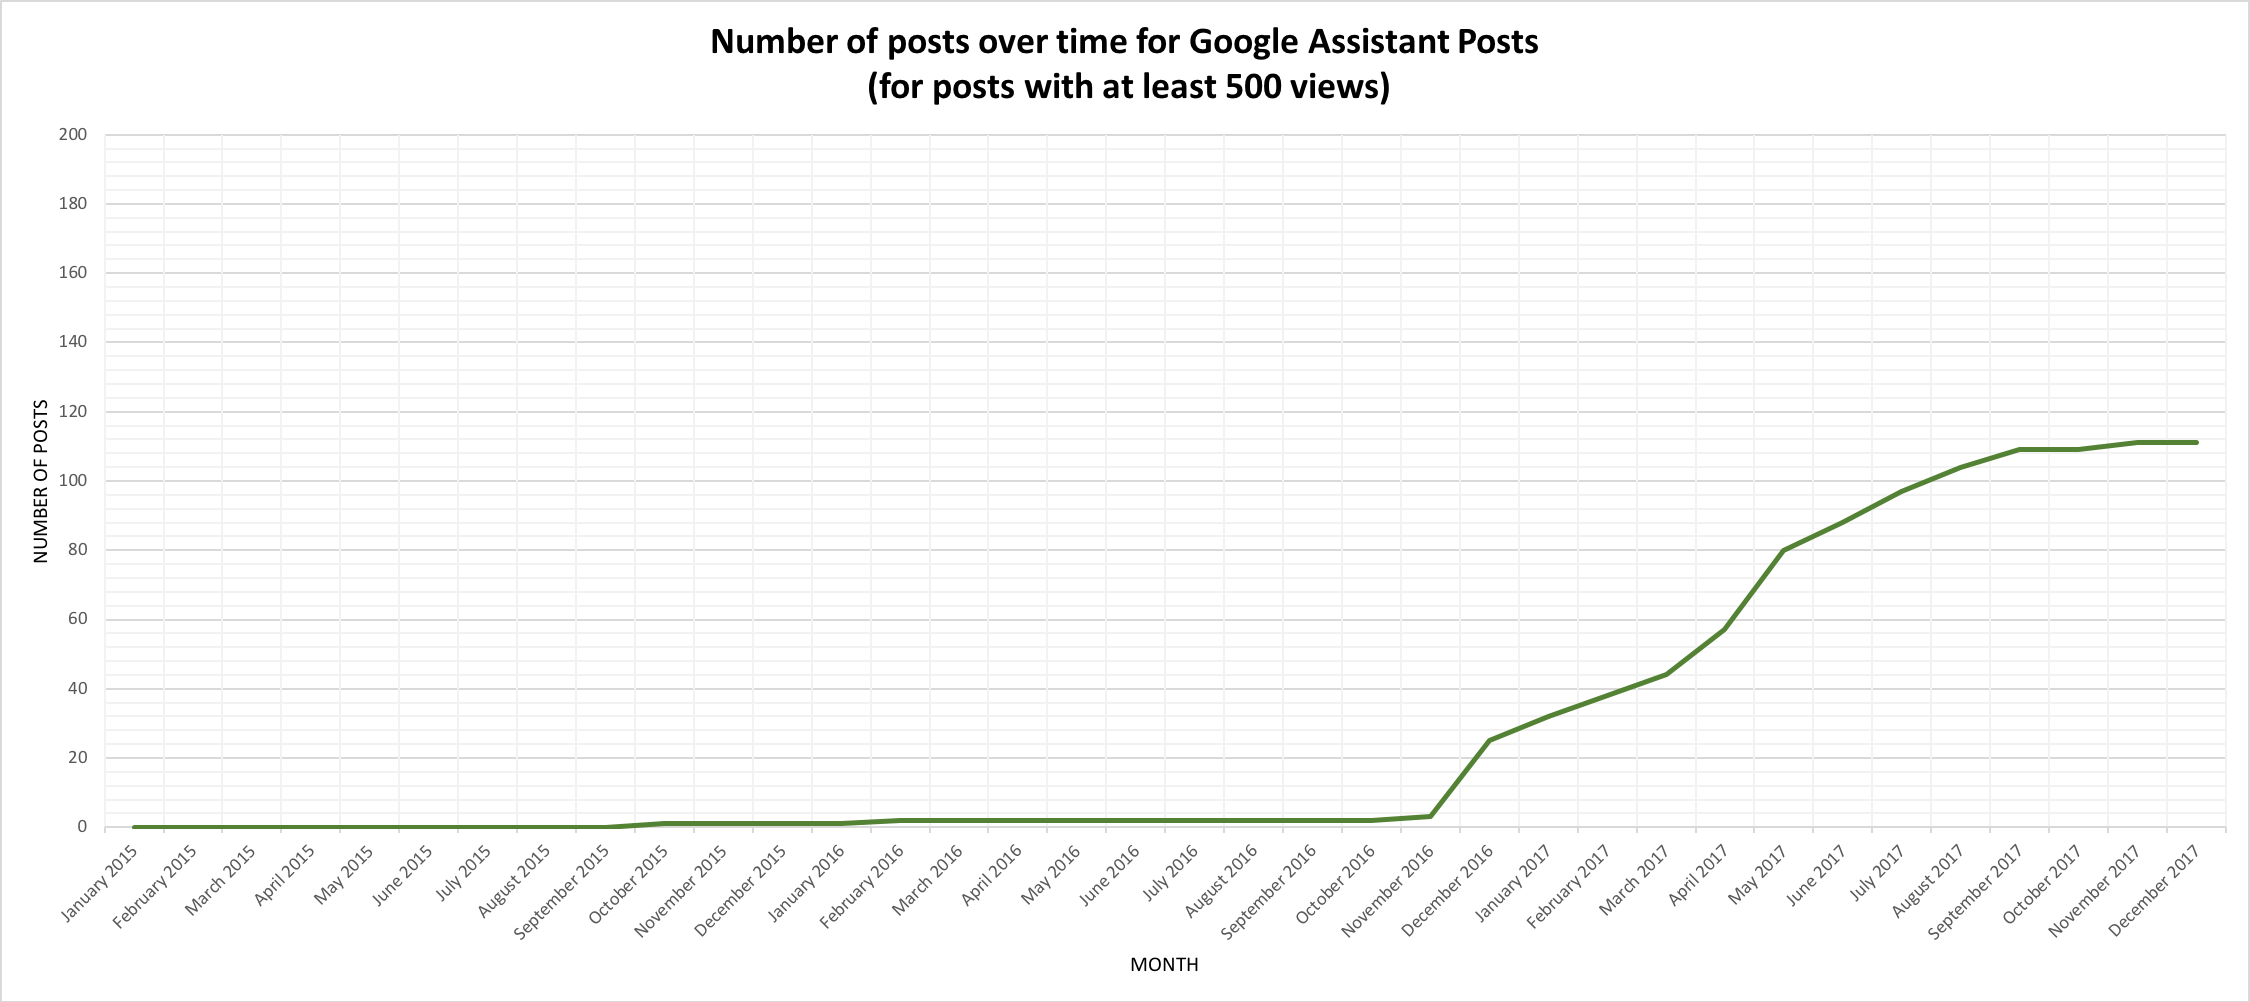
\includegraphics[width=\textwidth,height=\textheight,keepaspectratio]{RQ6-GoogleNumPostsOverTime_500Views.png}
    \caption{Growth in the number of posts over time for posts on Google Assistant, based on posts with at least 500 views}
    \label{fig:9GAGrowthInNumPosts500Views}
\end{figure}
\begin{figure}[ht]
	\centering
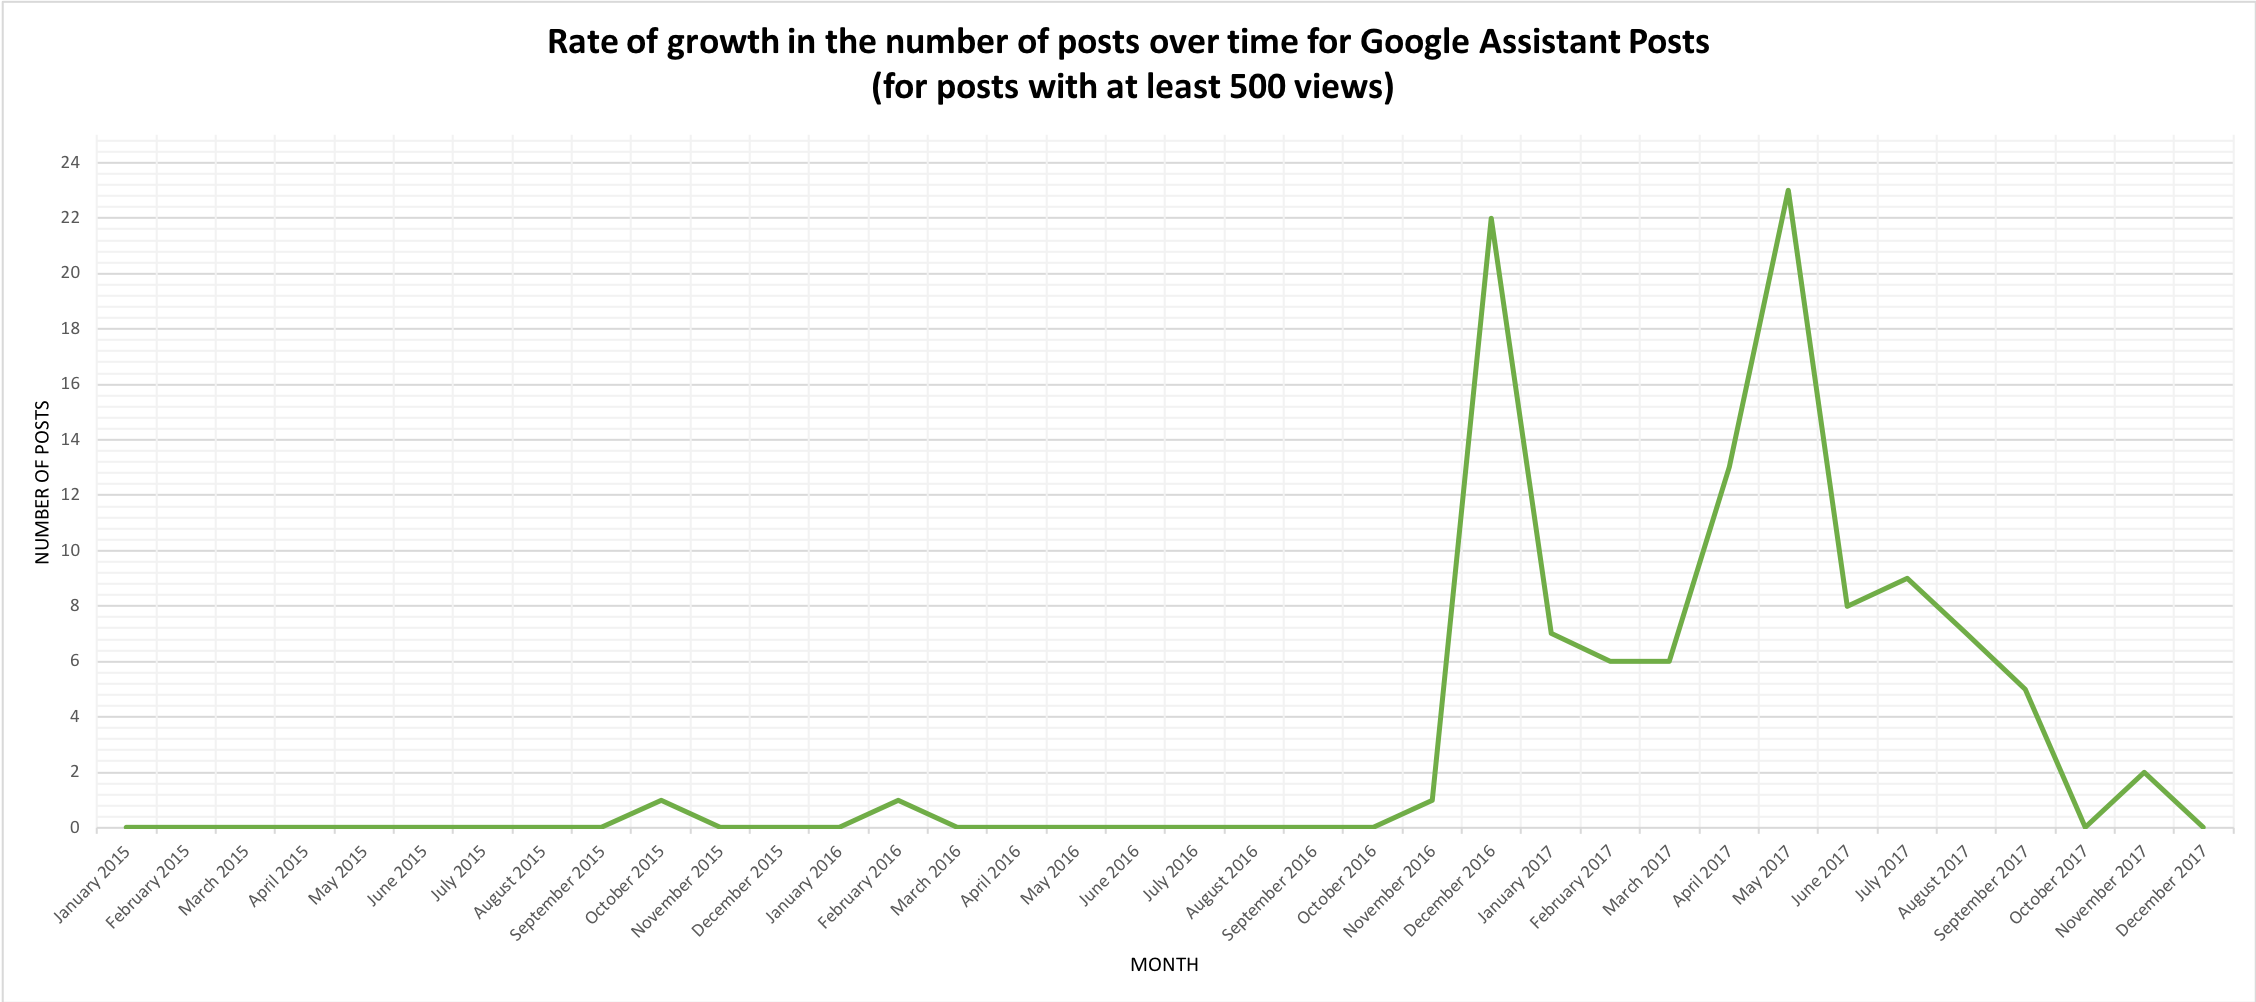
\includegraphics[width=\textwidth,height=\textheight,keepaspectratio]{RQ6-GoogleRateNumPostsOverTime_500Views.png}
    \caption{Rate of Growth in the number of posts over time for posts on Google Assistant, based on posts with at least 500 views}
    \label{fig:9.1GARateGrowthInNumPosts500Views}
\end{figure}

\begin{figure}[ht]
	\centering
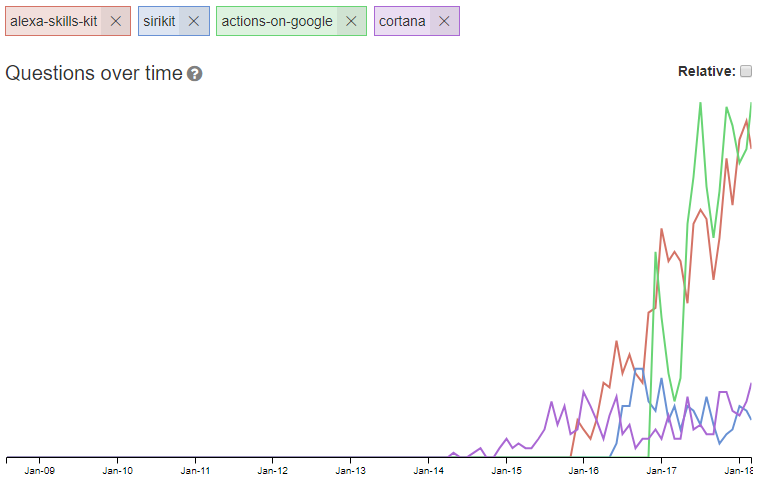
\includegraphics[scale=0.7]{RQ6_Tag_Trends_AGS.PNG}
    \caption{Number of posts created each month on StackOverflow for each of the VAs: Alexa, Google Home and Siri ( Most relevant tags based on number of views and posts.}
    \label{fig:11MonthlyPostsforAGSC}
\end{figure}



 %end of carryover%


%


 \end{document}